\documentclass[journal,twoside,web]{ieeecolor}
\usepackage{jsen}
\usepackage{cite}
\usepackage{amsmath,amssymb,amsfonts}
\usepackage{algorithmic}
\usepackage{graphicx}
\usepackage{textcomp}
\usepackage{wrapfig}
\usepackage{orcidlink}
\usepackage{comment}
\usepackage{stfloats}
\usepackage{url}
\usepackage{verbatim}
\usepackage{tabularx}
\usepackage{booktabs}
\usepackage{svg}


\def\BibTeX{{\rm B\kern-.05em{\sc i\kern-.025em b}\kern-.08em
    T\kern-.1667em\lower.7ex\hbox{E}\kern-.125emX}}
\markboth{\journalname, VOL. XX, NO. XX, XXXX 2024}
{Author \MakeLowercase{\textit{et al.}}: Preparation of Papers for IEEE TRANSACTIONS and JOURNALS (May 2024)}
\definecolor{abstractbg}{rgb}{0.89804,0.94510,0.83137}
\setlength{\fboxrule}{0pt}
\setlength{\fboxsep}{0pt}

\begin{document}
\title{Improving Generalization of EMI-Based Corrosion Quantification via Physics-Informed Features from Piezoelectric Self-Sensing Using the Butterworth–Van Dyke Model}
\author{Mads Kofod Dahl\orcidlink{0009-0006-4330-6730}, \IEEEmembership{Student Member, IEEE}, Raymond Houe Ngouna\orcidlink{0000-0003-2468-3283} ,Jaamac Hassan Hire\orcidlink{0000-0002-3714-7773}, \\Farshad Moradi, \IEEEmembership{Senior Member, IEEE}, Micky Rakotondrabe\orcidlink{0000-0002-6413-7271}, \IEEEmembership{Senior Member, IEEE}.
\thanks{Submitted for review \date{18-05-2026}. This work was supported by Innovationsfonden through the CORROSENSE Project under Grant 2081-00027A. Website: \url{https://corrosense.dk/}}
\thanks{Mads Kofod Dahl and Jaamac Hassan Hire are with the Department of Electrical and Computer Engineering, Aarhus University, 8200 Aarhus, Denmark. Farshad Moradi is with Microelectronics, Department of Mechanical and Electrical Engineering, University of Southern Denmark, 5230 Odense, Denmark and Micky Rakotondrabe and Raymond Houe Ngouna are with University of Technology of Tarbes Occitanie Pyrénées, 65000 Tarbes, France.}}

\IEEEtitleabstractindextext{%
\fcolorbox{abstractbg}{abstractbg}{%
\begin{minipage}{\textwidth}%
    \begin{wrapfigure}[18]{r}{3.0in}%
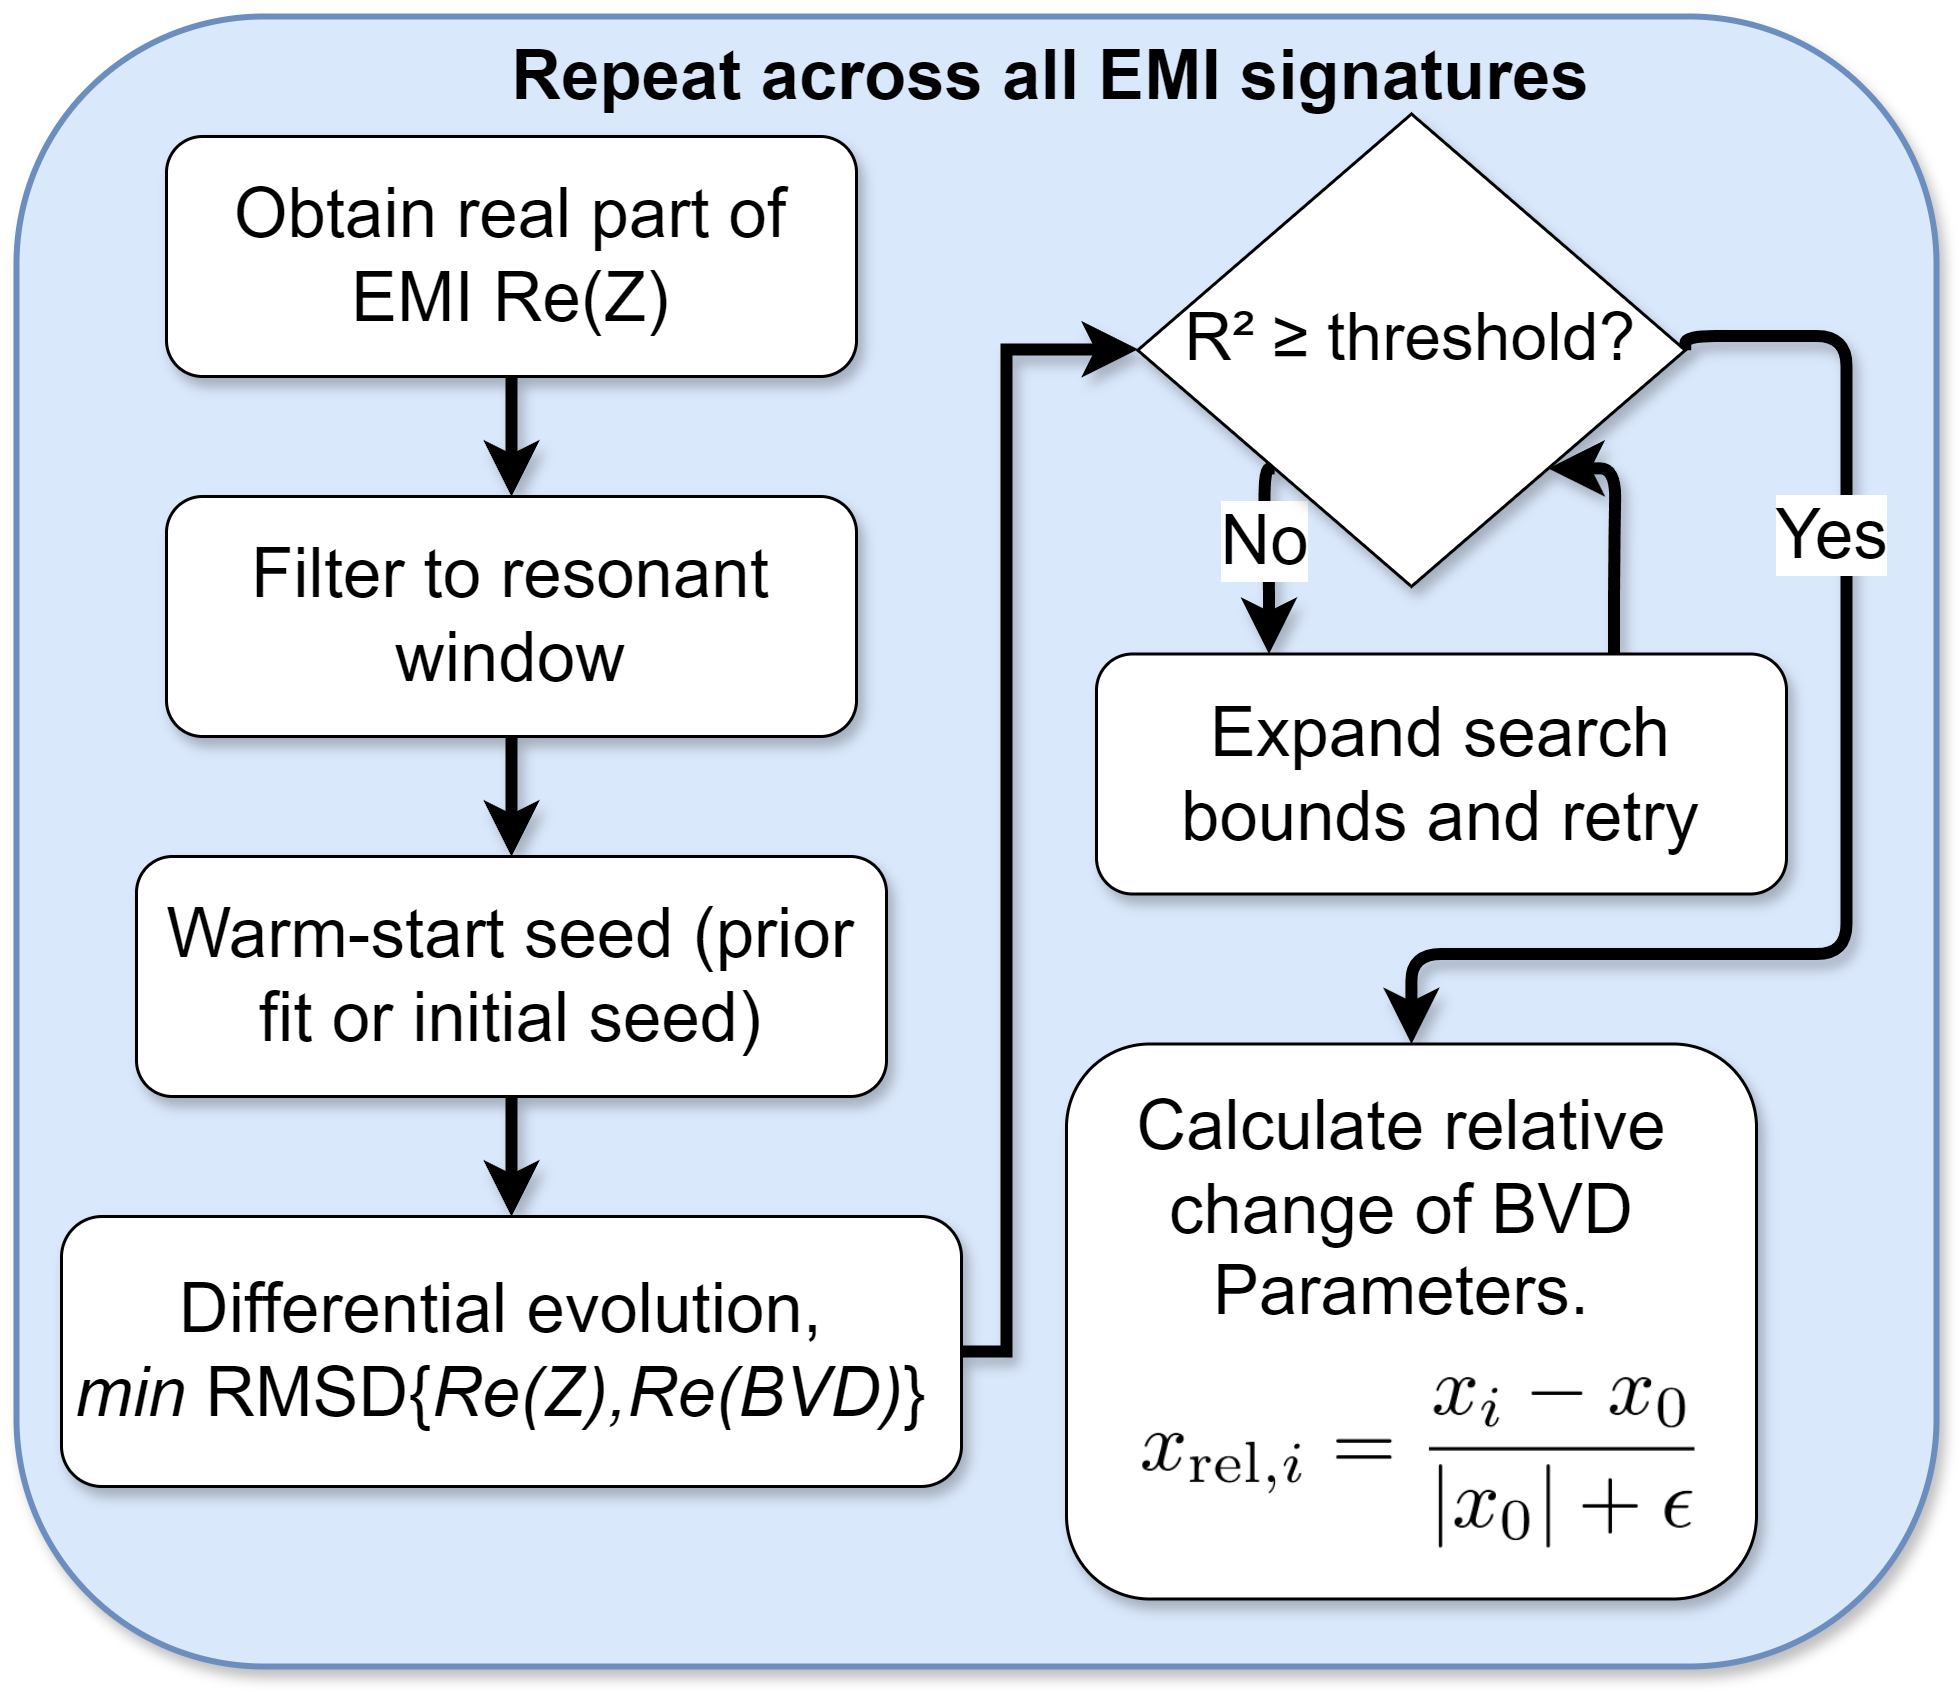
\includegraphics[width=2.6in]{images/EMI_BVD_Feature_Flowchart.drawio.png}%
\end{wrapfigure}%
\begin{abstract}
The electromechanical impedance (EMI) method is a promising, piezoelectric--based, technique for structural health monitoring. However, machine learning models trained on raw impedance data often fail to generalize to unseen samples. This paper proposes a physics-informed feature extraction approach based on the Butterworth--Van Dyke (BVD) equivalent circuit model to address this limitation. By fitting a constrained BVD circuit to the measured impedance signature, the high-dimensional impedance data is compressed into five physically meaningful parameters. Three steel samples undergoing accelerated galvanic corrosion were used to evaluate the approach under leave-one-out (LOO) cross-validation, where each model predicts mass loss on a sample not seen during training. A Convolutional Neural Network trained on BVD features achieved average training and validation RMSE scores of 3.31\,g and 2.51\,g, respectively, across approximately 40\,g of total mass loss, outperforming an equivalent model trained directly on raw impedance spectra, demonstrating improved generalization across previously unseen samples. In this paper we demonstrate that the proposed feature extraction approach improves cross-sample robustness in corrosion quantification from EMI data. The proposed approach is directly applicable to structural health monitoring of reinforced concrete, where sacrificial EMI sensor probes are used to monitor corrosion of steel reinforcement.
\end{abstract}

\begin{IEEEkeywords} Electromechanical impedance, structural health monitoring, corrosion quantification, Butterworth--Van Dyke model, physics-informed feature extraction, neural network, piezoelectric self-sensing.
\end{IEEEkeywords}
\end{minipage}}}

\maketitle

\section{Introduction}\label{sec:introduction}
\IEEEPARstart{S}{tructural} health monitoring (SHM) enables the continuous assessment of engineering structures, allowing early detection of damage before catastrophic failure occurs. 

%SHM is commonly described in terms of four hierarchical levels: Level \RomanNumeralCaps{1} damage detection, Level \RomanNumeralCaps{2} damage localization, Level \RomanNumeralCaps{3} damage assessment or quantification, and Level \RomanNumeralCaps{4} remaining useful life estimation. The levels represent progression from identifying the presence of damage to characterizing its severity and ultimately predicting future structural performance. Within this framework, different sensing modalities and analysis methods can be evaluated based on the level of insight they provide.

In civil infrastructure, a major application of SHM is the monitoring of reinforced concrete structures, where corrosion of embedded steel reinforcement is a primary cause of long-term deterioration. Corrosion leads to progressive loss of cross-sectional area, cracking, and stiffness degradation, ultimately compromising structural integrity. Reliable methods for early detection and quantification of corrosion are therefore essential for maintaining safety and enabling predictive maintenance strategies.

Among the available SHM techniques, the electromechanical impedance (EMI) method has attracted considerable attention due to its sensitivity to incipient structural changes and its relatively simple instrumentation requirements\cite{ren2025_damage_detection_shm}. In the EMI technique, a piezoelectric patch, commonly a lead-zirconate-titanate (PZT) piezo, is bonded onto the structure and acts as both actuator and sensor. Such use of piezoelectric patches for simultaneous actuation and measurement is also called piezoelectric self-sensing and was investigated previously for vibration damping and for robotic manipulation \cite{SSMech10,SSTmech15,SSTIE17,SSSNA26}. In this paper, piezoelectric self-sensing is used to obtain EMI data and use apply it to the task of corrosion monitoring. To this aim, an alternating voltage excites the piezoelectric patch, and the resulting electrical impedance is measured across a range of frequencies, typically $50$kHz to $500$kHz. Because the electrical impedance is coupled to the mechanical impedance of the host structure, any changes in structural properties alters the measured EMI signature.

The analytical model proposed by Liang et al.\ \cite{liang_1994} formalizes this coupling by relating the mechanical impedance of the PZT patch ($Z_T(\omega)$) and that of the host structure ($Z_S(\omega)$) to the complex electrical admittance ($\bar{Y}$) at the PZT patch terminals:

\begin{equation}
\begin{split}
    \overline{Y} &= \omega j \frac{wl}{h} \left[ \left( \overline{\varepsilon^T_{33}} - d^2_{31} \overline{Y^E} \right) \right. \\
    &\left. + \left( \frac{Z_T}{Z_S + Z_T} \right) d_{31}^2 \overline{Y^E} \left( \frac{\tan(\kappa l)}{\kappa l} \right) \right]
\end{split}
\label{eq:EMIA}
\end{equation}

The corresponding electrical impedance is given by $Z = 1 / \bar{Y}$, where $w$, $h$, and $l$ are the width, height, and length of the PZT patch, $\varepsilon_{33}^T$ denotes the dielectric permittivity of the PZT patch, $d_{31}$ the transversal piezoelectric constant, $Y^E$ the complex Young's modulus, and $\kappa$ the one-dimensional wave number associated with the angular frequency $\omega$.

This relationship links the EMI signature to the mechanical and electrical properties of both the device under test (DUT) and the PZT patch through $Z_S(\omega)$ and $Z_T(\omega)$. Because the mechanical impedance of the PZT patch is much smaller than that of the DUT, variations in the electrical impedance mainly reflect changes in the mechanical impedance of the host structure, providing a basis for detecting structural damage. The impedance of the host structure can be described by:

\begin{equation}
Z_S = c + m\mathrm{j}\omega + \frac{k}{\mathrm{j}\omega}
\label{eq:blockImpedance}
\end{equation}

where $m$, $k$, and $c$ represent effective mass, stiffness, and damping, respectively.

Damage detection is conventionally performed by comparing the real part of the EMI signature in a healthy (reference) state with that in a potentially damaged state, using a metric such as the Root Mean Squared Deviation (RMSD) \cite{na2018review}. The RMSD quantifies deviations between reference and subsequent measurements and is defined as:

\begin{equation}
\mathrm{RMSD}=\sqrt{\frac{\sum_{i=1}^{N} \left( R_D(i) - R_{\mathrm{Ref}}(i) \right)^2
}{\sum_{i=1}^{N} \left( R_{\mathrm{Ref}}(i) \right)^2}}
\label{eq:rmsd}
\end{equation}

where $i$ denotes the $i$-th data point of the EMI signature, $N$ is the total number of data points, $R_{\mathrm{Ref}}$ is the real part of the impedance in the reference state, and $R_D$ represents the real part of the impedance in a subsequent measurement.

In general, damage progression manifests as a shift in the resonance frequency and changes in peak magnitude due to modified mass, damping, and stiffness of the host structure. The RMSD algorithm is commonly used to detect the presence of damage and using the unitless RMSD number as a deviation metric to distinguish damaged from undamaged states ~\cite{NA_res_dmg}. Alongside this, considerable effort has gone into understanding the influence of ambient conditions on the EMI signature, particularly temperature has received attention ~\cite{park1999temperature, shelgaonkar2025_thermal_emi_shm}, in our previous work we investigated the effects of both temperature ~\cite{Dahl_multi_model} and humidity ~\cite{Dahl_humid}. 

Methods for damage localization have also been proposed~\cite{ZHU2021107001, pereira2024damage, djemana2017}, yet while detection and localization are increasingly well addressed, accurate damage quantification—estimating how much or the type of damage that has occurred—remains understudied. The RMSD, despite its popularity, does not reliably serve this purpose: as shown in Section~\ref{sec3}, it can fluctuate substantially and yield similar values for very different levels of mass loss, making it unsuitable for continuous quantitative damage tracking over time.

The EMI method and RMSD algorithm has been shown to be able to detect damage, but exact damage quantification remains a challenge. The present work addresses this gap by seeking to establish a more consistent relationship between EMI-derived features and the structural parameters of mass, stiffness and damping.


\subsection{Machine Learning for EMI-Based Damage Quantification in Reinforced Concrete and Steel Structures}

To improve damage detection and quantification methods, several authors have investigated applying machine learning (ML) to EMI signatures. Table~\ref{tab:emi_concrete_corrosion} summarizes representative studies in which ML models were trained on EMI data for damage assessment in concrete and steel structures.

\begin{table*}[h!]
\centering
\small
\caption{Representative studies applying ML to EMI-based damage assessment.}
\label{tab:emi_concrete_corrosion}
\begin{tabularx}{\textwidth}{lll X X X}
\toprule
Ref. & Target & Method & Classification type & Key approach & Results\\
\midrule
\cite{ai2023} & Concrete & 2D CNN & Five mass-loss damage scenarios & Damage quantification from EMI using a two-dimensional convolutional network. & PZT patch placed on the outside of concrete, minimum mass loss: 184\,g\\
\cite{li2021} & Concrete & 1D CNN & Twelve cases with different crack depths and temperatures & EMI-based concrete damage quantification under variable temperature conditions. & PZT patch placed on the outside of concrete, minimum crack depth: 10\,mm\\
\cite{bansal2022} & Curing & SVM & Compressive strength & Prediction of concrete compressive strength using piezoelectric sensor EMI data. & Strength increase during curing, piezo outside of concrete\\
\cite{luo2022} & Corrosion & 1D CNN & Mass loss caused by pitting corrosion & Pitting corrosion mass-loss prediction by combining EMI measurements with CNN. & 2.6\% to 30\% mass loss, pitting corrosion, on top of steel\\
\cite{li2023} & Concrete & LR-CNN & Compressive strength & Early-age concrete strength monitoring using smart aggregates. & Strength curing, inside concrete\\
%\cite{park2008electro} & Bolts & PCA/K-means & Bolt loosening & Applies RMSD on PCA-compressed data and uses K-means clustering to identify damage. & ---\\
\bottomrule
\end{tabularx}
\end{table*}

\subsubsection{PZT Placement}

In many studies, a PZT patch is mounted on the surface of concrete, such that damage is typically detected only after visible cracking has already occurred. To increase sensitivity to early damage, the PZT patch can be bonded directly to exposed rebar or to a sacrificial steel probe embedded in the RC. This enables more direct monitoring of the corrosion processes, the primary mechanism driving long-term structural degradation in RC structures. In this work we evaluate the effect of corrosion on PZT sensors bonded to sacrificial steel probes designed to be embedded in RC.

\subsubsection{ML Evaluation}

Beyond sensor placement, limitations also arise from how ML models are trained and evaluated. Many studies rely on standard train–test splits or K-fold cross-validation using data from the same sample or a relatively small set of samples. Under these conditions, models may learn sample-specific characteristics rather than generalizable patterns. This reduces their applicability in real-world SHM scenarios, where predictions must be made on previously unseen structures.

As demonstrated in this work, machine learning models trained directly on raw or relative impedance data often struggle to generalize, as EMI signatures are highly sensitive to sample-specific factors such as geometry, bonding conditions, and PZT patch placement. Even minor variations can lead to significant differences in impedance responses.

Demonstrating true generalization requires large and diverse datasets; however, few high-quality EMI datasets are publicly available. Therefore we suggest that, leave-one-out (LOO) cross-validation will provide a more rigorous alternative to standard train-test splits. By training on all but one sample and testing on the excluded sample, a well preforming model can be said to better capture the patterns of the underlying damage effects instead of sample specific damage markers.


\subsection{Physics-informed BVD feature extraction}

To address the problem of generalization, we propose using the Butterworth--Van Dyke (BVD) equivalent circuit model as a physics-informed, feature extraction step, prior to neural network training. While baseline-free EMI methods that extract physical properties from resonance peaks have been explored for concrete modulus estimation~\cite{sha2024baseline}, physics-informed feature extraction for damage quantification remains unaddressed. The BVD circuit was originally developed to model piezoelectric resonators near their resonance frequency. As seen in figure \ref{fig:BVD-model-and-impedance}.A the BVD model consists of a motional branch ($R_1$, $L_1$, $C_1$ in series) in parallel with a static capacitance $C_0$\cite{BVD}. We add an additional series resistance $R_0$, to model the resistance of the wires and the bonding layer. Figure \ref{fig:BVD-model-and-impedance}.B shows the complex, frequency dependent impedance ($Z(\omega)$) of the BVD circuit in series with $R_0$ and is given by:

\begin{equation}
    Z(\omega) = R_0 + \left(\mathrm{j} \omega C_0 + \frac{1}{R_1 + \mathrm{j}\omega L_1 + \frac{1}{\mathrm{j}\omega C_1}}\right)^{-1}
    \label{eq:BVD-Z}
\end{equation}

% This is kind of true but I only kind of use this fact, maybe it is okay to keep as a step in the argument for why BVD is better than raw features, but I don't want to overstate it. Especially since I only have the actual mass change not stiffness of damping so.
The BVD model can be mapped to an equivalent mechanical mass--spring--damper system where $L_1$ corresponds to the effective mass, $C_1$ to the mechanical compliance (inverse stiffness), and $R_1$ to damping. This interpretation provides a direct physical link between circuit parameter variations and structural changes. In particular, corrosion-induced mass loss is expected to reduce $L_1$, while changes in stiffness and damping manifest as variations in $C_1$ and $R_1$, respectively. By fitting a BVD circuit to each measured EMI signature, the high-dimensional impedance data is compressed into five physically meaningful circuit parameters $R_0$, $R_1$, $L_1$, $C_1$, and $C_0$. 

%To further incorporate prior knowledge, a monotonic decrease constraint is imposed on $L_1$ during the fitting process, this reflects the expected mass reduction due to progressive corrosion. Furthermore the initial value of $L_1$ is set to $20$ mH reflecting a known initial mass. 

%The full pipeline can be seen in figure \ref{fig:ML-diagram}, which shows the real part of the impedance data being obtained over time ($\text{Re}(Z,t)$), BVD parameters are fitted such that $\text{RMSD} (\text{Re} (Z,t) - \text{Re} (Z_{BVD},t))$ is minimized. The relative change in the BVD parameters ($rel\_R_0, rel\_R_1, rel\_L_1, rel\_C_1, rel\_C_0$) is then used as input features for the neural network. The BVD fitting serves as a feature extraction step that strips away sample-specific details while preserving the damage-related information encoded in the behavior of the main resonance.

\begin{figure}[!t]
    \centering
    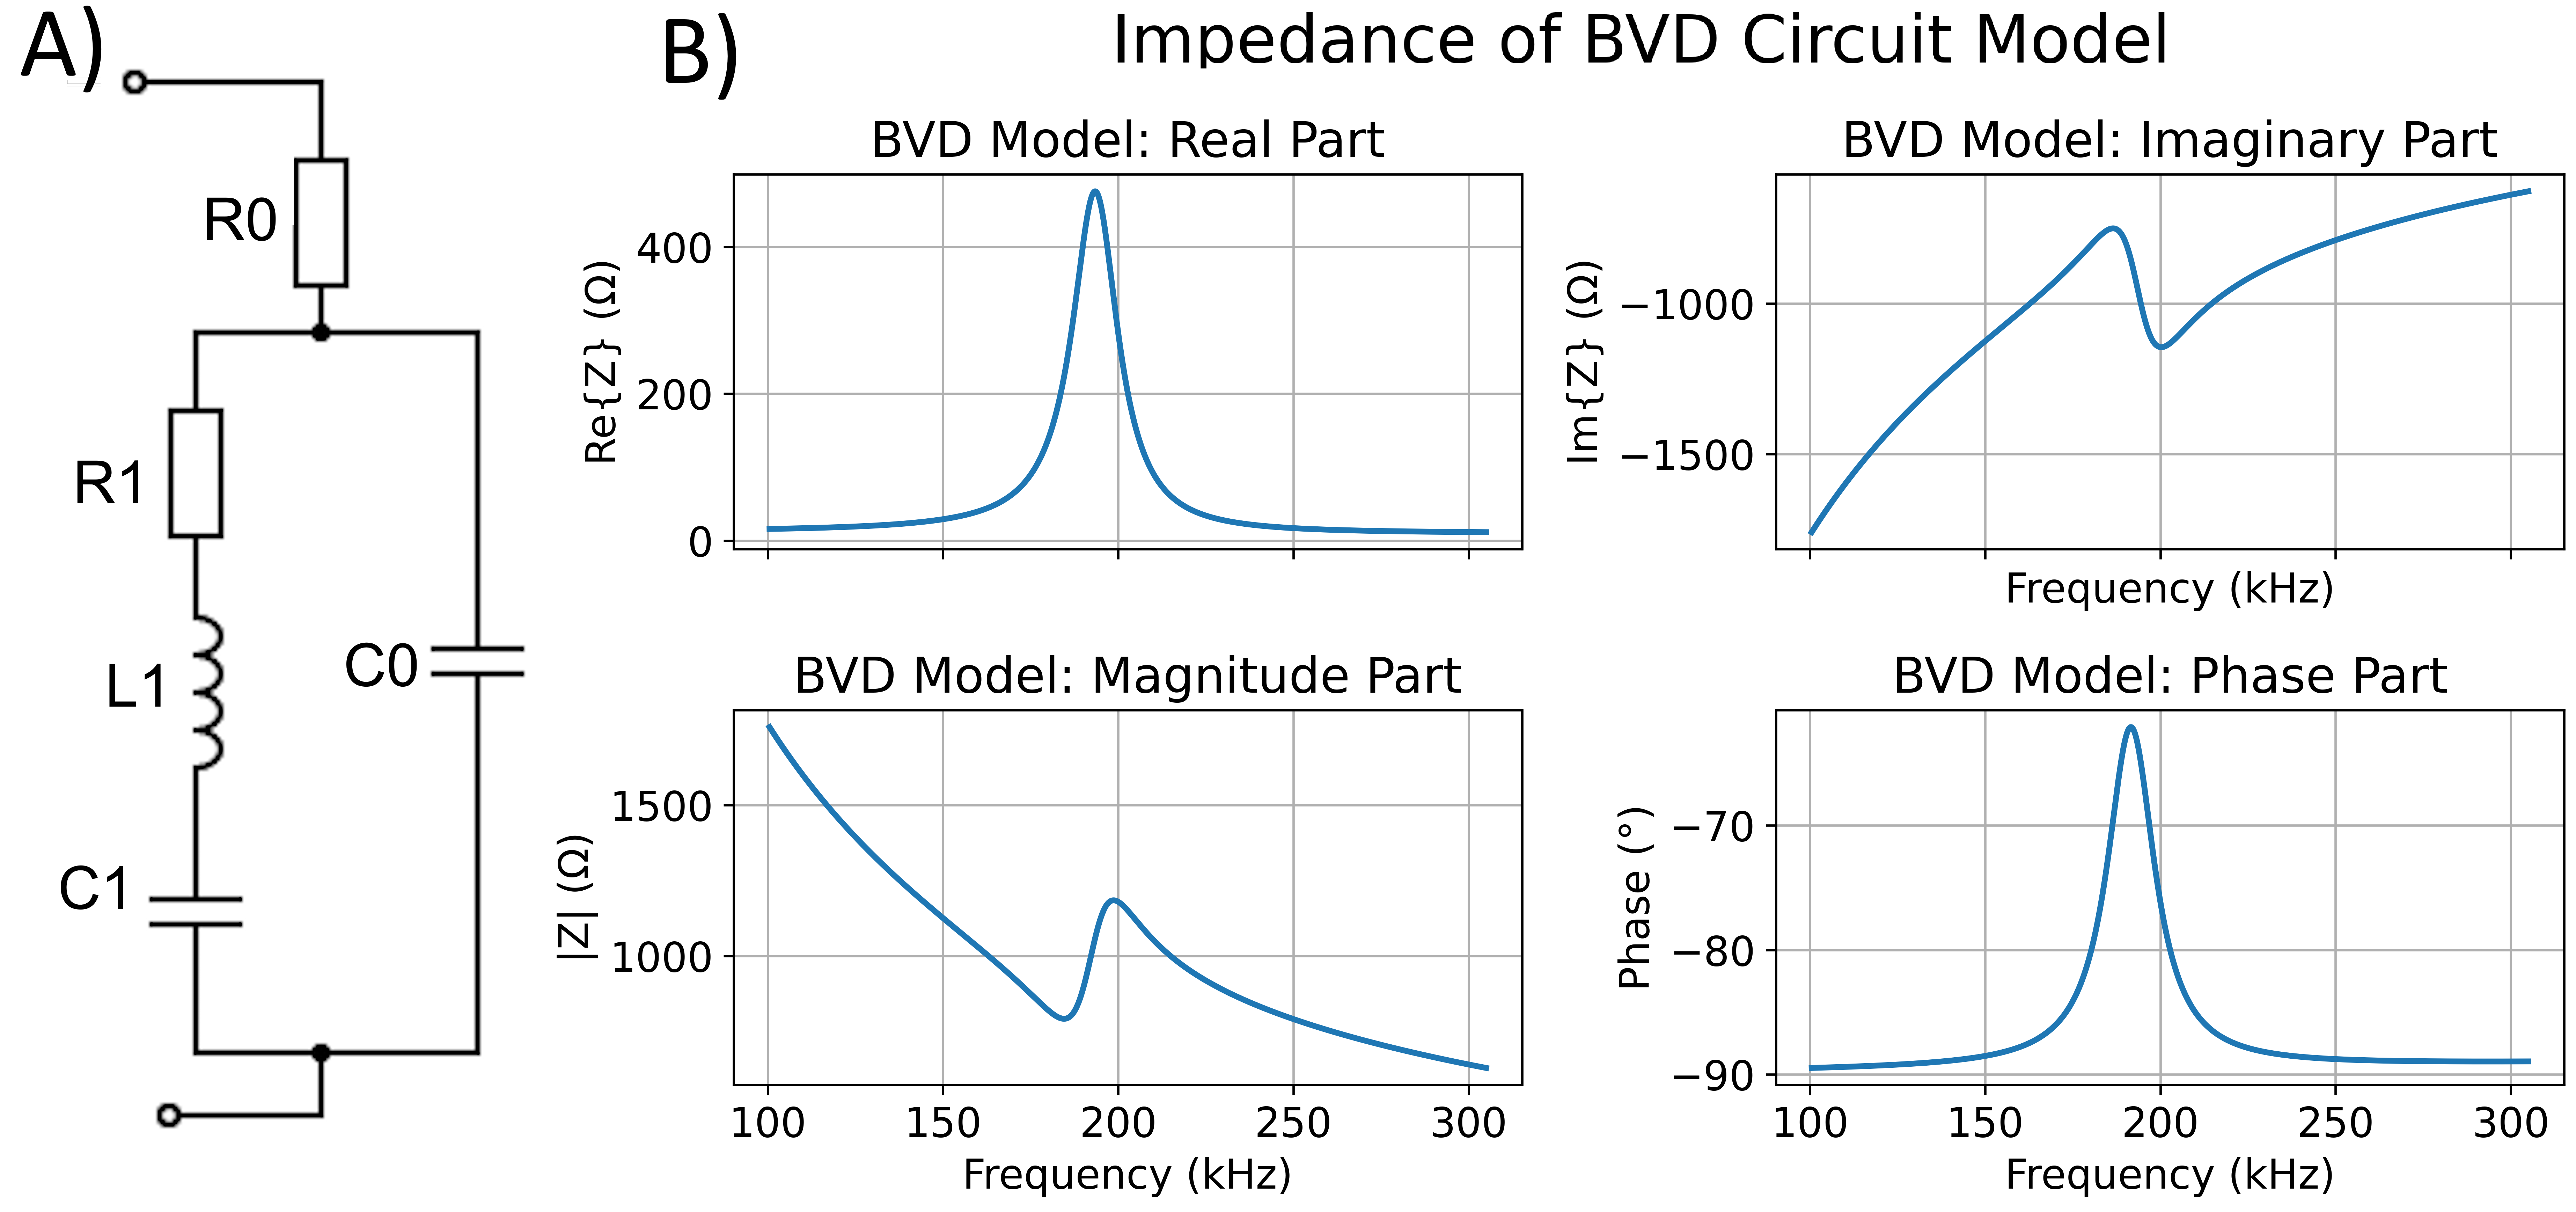
\includegraphics[width=1\linewidth]{images/BVD-circuit-and-impedance.png}
    \caption{A) Augmented Butterworth--Van Dyke (BVD) equivalent circuit with series resistance $R_0$, motional branch ($R_1$, $L_1$, $C_1$), and static capacitance $C_0$. B) Example BVD model fit to the real part of a measured EMI signature near the main resonance peak.}
    \label{fig:BVD-model-and-impedance}
\end{figure}

\subsection{Contributions}

The main contributions of this work are as follows:
\begin{enumerate}
    \item We show that neural networks trained directly on raw or relative impedance data fail to generalize under leave-one-out (LOO) cross-validation, highlighting a key limitation of existing machine learning approaches for EMI-based damage quantification.
    
    \item We propose a physics-informed feature extraction method based on constrained Butterworth–Van Dyke (BVD) circuit fitting, which compresses high-dimensional EMI signatures into a small set of physically interpretable parameters.
    
    \item We validate the proposed approach on three steel specimens undergoing accelerated corrosion, demonstrating that a BVD-informed neural network outperforms models trained on raw and impedance features in predicting mass loss for unseen specimens. These steel samples are representative of sacrificial EMI probes for use in corrosion monitoring in reinforced concrete structures.
\end{enumerate}

The remainder of this paper is organized as follows. Section~\ref{sec2} describes the sample preparation, experimental setup, and ML model training. Section~\ref{sec3} presents the results and evaluates the performance of the different models. Section~\ref{sec4} discusses the findings and limitations. Section~\ref{sec5} concludes the paper.

%%%%%%%%%%%%%%%%%%%%%%%%%%%%%%%%%%%%%%%%%%%%%%%%%%%%%%%%%%%%%%%%%

\section{Methods}\label{sec2}

This section describes the sample design, experimental setup for accelerated corrosion and impedance acquisition, the BVD-based feature extraction procedure, and the neural network architectures used for mass-loss prediction.

\subsection{Samples}

Three cylindrical steel samples were fabricated with identical geometry. Each sample has two narrowed ends that are 25\,mm long and 10\,mm in diameter, with a square recess of $11 \times 10$\,mm machined into one end to accommodate the PZT patch. The central section of the sample is 50\,mm long and 16\,mm in diameter. The reduced cross-section at the ends promotes stronger mechanical resonance peaks due to the cantilever effect. The reduced diameter of the ends also allows for the application of a silicone protective layer of 6\,mm diameter around the PZT.
% TODO: add patent reference for the thinner-end design

A $10mm \times 10mm \times 1 mm$, PZT patch (APC 840, from American Piezo Ceramics) was bonded to one end of each steel sample using CW2400 conductive epoxy (Chemtronics)\cite{CW2400}. The positive lead was soldered directly to the PZT patch, and the negative lead was attached to the steel surface using the same conductive epoxy. The material properties of the APC 840 ceramic are listed on the APC website\cite{apc_piezo_properties}.

\begin{comment}
    
\begin{table}[ht]
\centering
\small
\begin{tabular}{lc}
\hline
\textbf{Parameter} & \textbf{APC 840} \\
\hline
Navy Type Equivalent & Navy I \\
\hline
\multicolumn{2}{l}{\textit{Dielectric Properties}} \\
$K_T$ & 1275 \\
$\tan \delta$ (\%) & 0.60 \\
$T_c$ (°C) & 325 \\
\hline
\multicolumn{2}{l}{\textit{Electromechanical Coupling}} \\
$k_p$ & 0.59 \\
$k_{33}$ & 0.72 \\
$k_{31}$ & 0.35 \\
$k_{15}$ & 0.70 \\
\hline
\multicolumn{2}{l}{\textit{Piezoelectric Charge Constants ($10^{-12}$ C/N)}} \\
$d_{33}$ & 290 \\
$-d_{31}$ & 125 \\
$d_{15}$ & 480 \\
\hline
\multicolumn{2}{l}{\textit{Piezoelectric Voltage Constants ($10^{-3}$ Vm/N)}} \\
$g_{33}$ & 26.5 \\
$-g_{31}$ & 11.0 \\
$g_{15}$ & 38.0 \\
\hline
\multicolumn{2}{l}{\textit{Elastic Properties ($10^{10}$ N/m$^2$)}} \\
$Y^E_{11}$ & 8.0 \\
$Y^E_{33}$ & 6.8 \\
\hline
\multicolumn{2}{l}{\textit{Frequency Constants (Hz$\cdot$m)}} \\
$N_L$ (longitudinal) & 1524 \\
$N_T$ (thickness) & 2005 \\
$N_P$ (planar) & 2130 \\
\hline
\multicolumn{2}{l}{\textit{Other Properties}} \\
$\rho$ (g/cm$^3$) & 7.6 \\
$Q_m$ & 500 \\
\hline
\end{tabular}
\caption{Material properties of APC 840 piezoelectric ceramic \cite{APC840}.}
\label{tab:APC-params}
\end{table}
\end{comment}

\begin{comment}
    

\begin{figure}[!t]
    \centering
    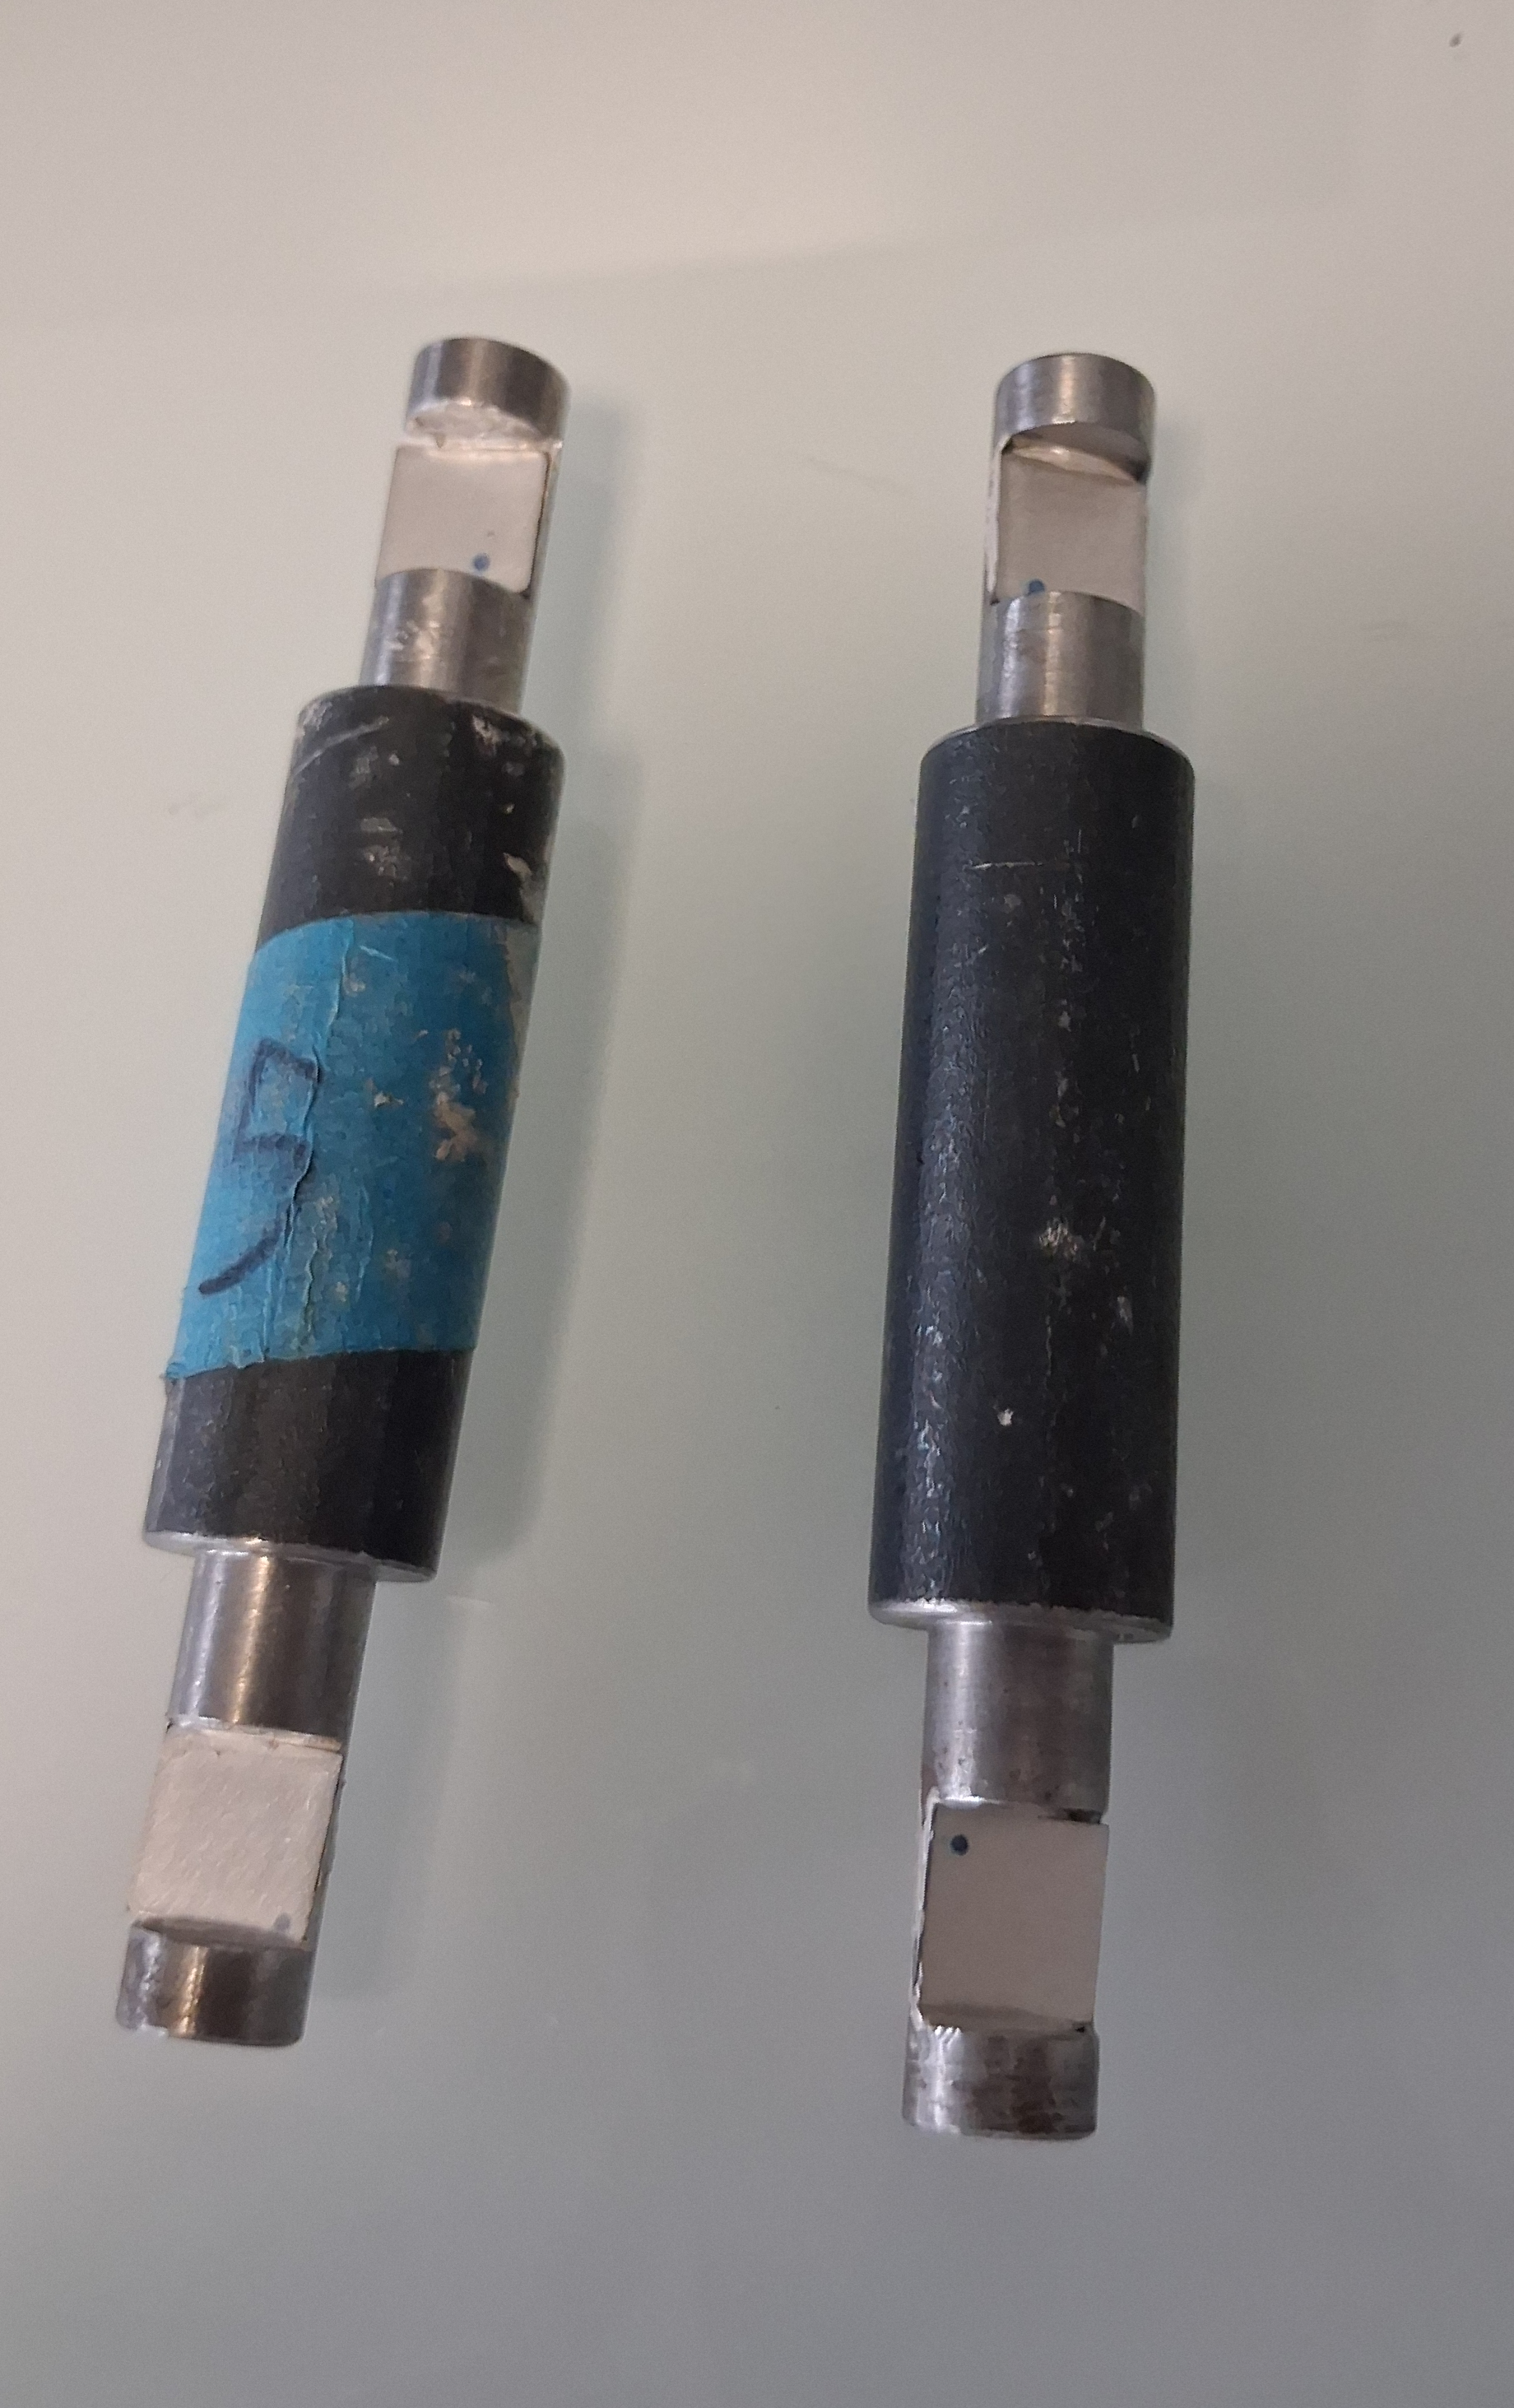
\includegraphics[width=0.4\linewidth]{images/Samples.png}
    \caption{Samples~1 and~2 with the PZT patch installed prior to lead wire attachment. (length$=100mm$)}
    \label{fig:samples}
\end{figure}

\end{comment}


\subsection{Experimental setup}\label{sec:data-collection}

The complex impedance of each sample was measured using a Zurich Instruments MFLI lock-in amplifier. The impedance was swept over a frequency range encompassing the main resonance peak: 180--205\,kHz for Samples~1 and~2, and 195--240\,kHz for Sample~3. To induce accelerated corrosion, the three samples were submerged in a 3\,\% NaCl (sodium chloride) solution together with a steel cathode. The PZT patches were kept above the waterline to avoid electrical shorts or PZT degradation. Each sample was connected to an individual channel of a power supply unit (PSU), current-limited to approximately 100\,mA. Each sample experienced approximately 766\,mV. The test setup is shown in Figs.~\ref{fig:Test-setup} and~\ref{fig:samples-in-water}.

% Mention that the PZTs are kept above the water to avoid shorts or corrosion on the PZT. In a real setup the PZT would be covered in a protective silicone layer.

Impedance measurements were taken approximately once per day over the course of the experiment, yielding 24 impedance datasets per sample (72 in total). At each measurement session, the air temperature and relative humidity were also recorded, and the galvanic current through each sample was verified to be stable. In addition, each sample was cleaned, dried and weighed seven times during the experiment to provide ground-truth mass-loss values for calibration (see Section~\ref{sec:mass-loss}).

As illustrated in Fig.~\ref{fig:Test-setup}, each sample has its own PSU channel with a common ground. The current path is as follows: from PSU Ch.~$x$ through the steel of sample~$x$, through the 3\% NaCl water solution to the steel cathode, and to common ground, where $x = 1, 2, 3$.

\begin{figure}[!t]
    \centering
    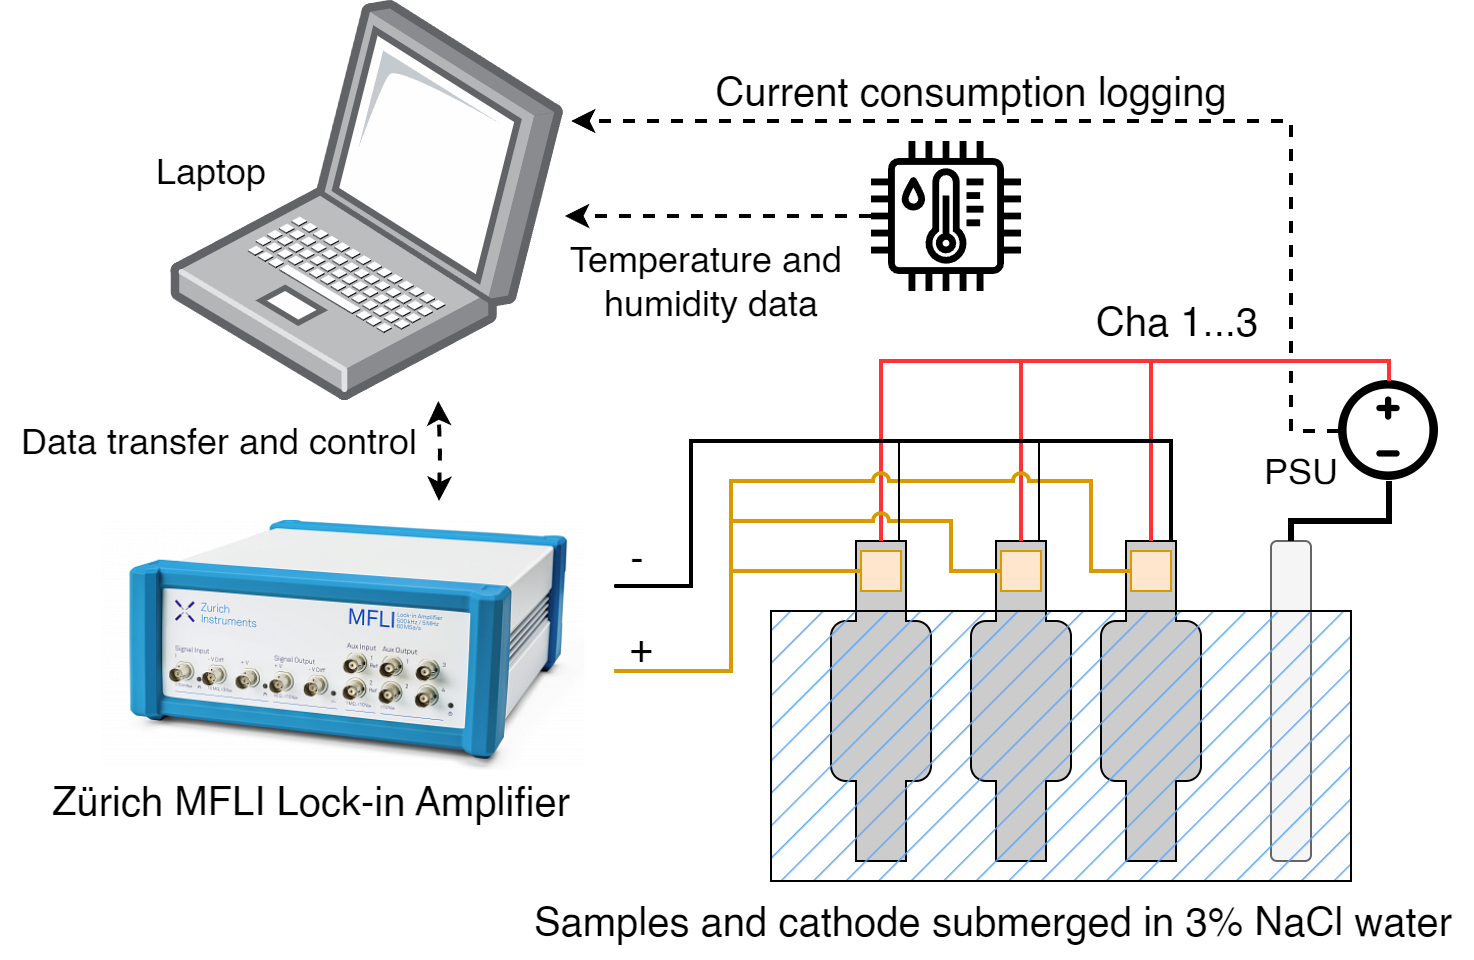
\includegraphics[width=1\linewidth]{images/Test-Setup-UTTOP.png}
    \caption{Experimental setup showing Samples~1--3 connected to the Zurich Instruments MFLI lock-in amplifier and the PSU. The PZT patches are kept above the water to avoid shorts or corrosion of the PZT.}
    \label{fig:Test-setup}
\end{figure}

\begin{figure}[!t]
    \centering
    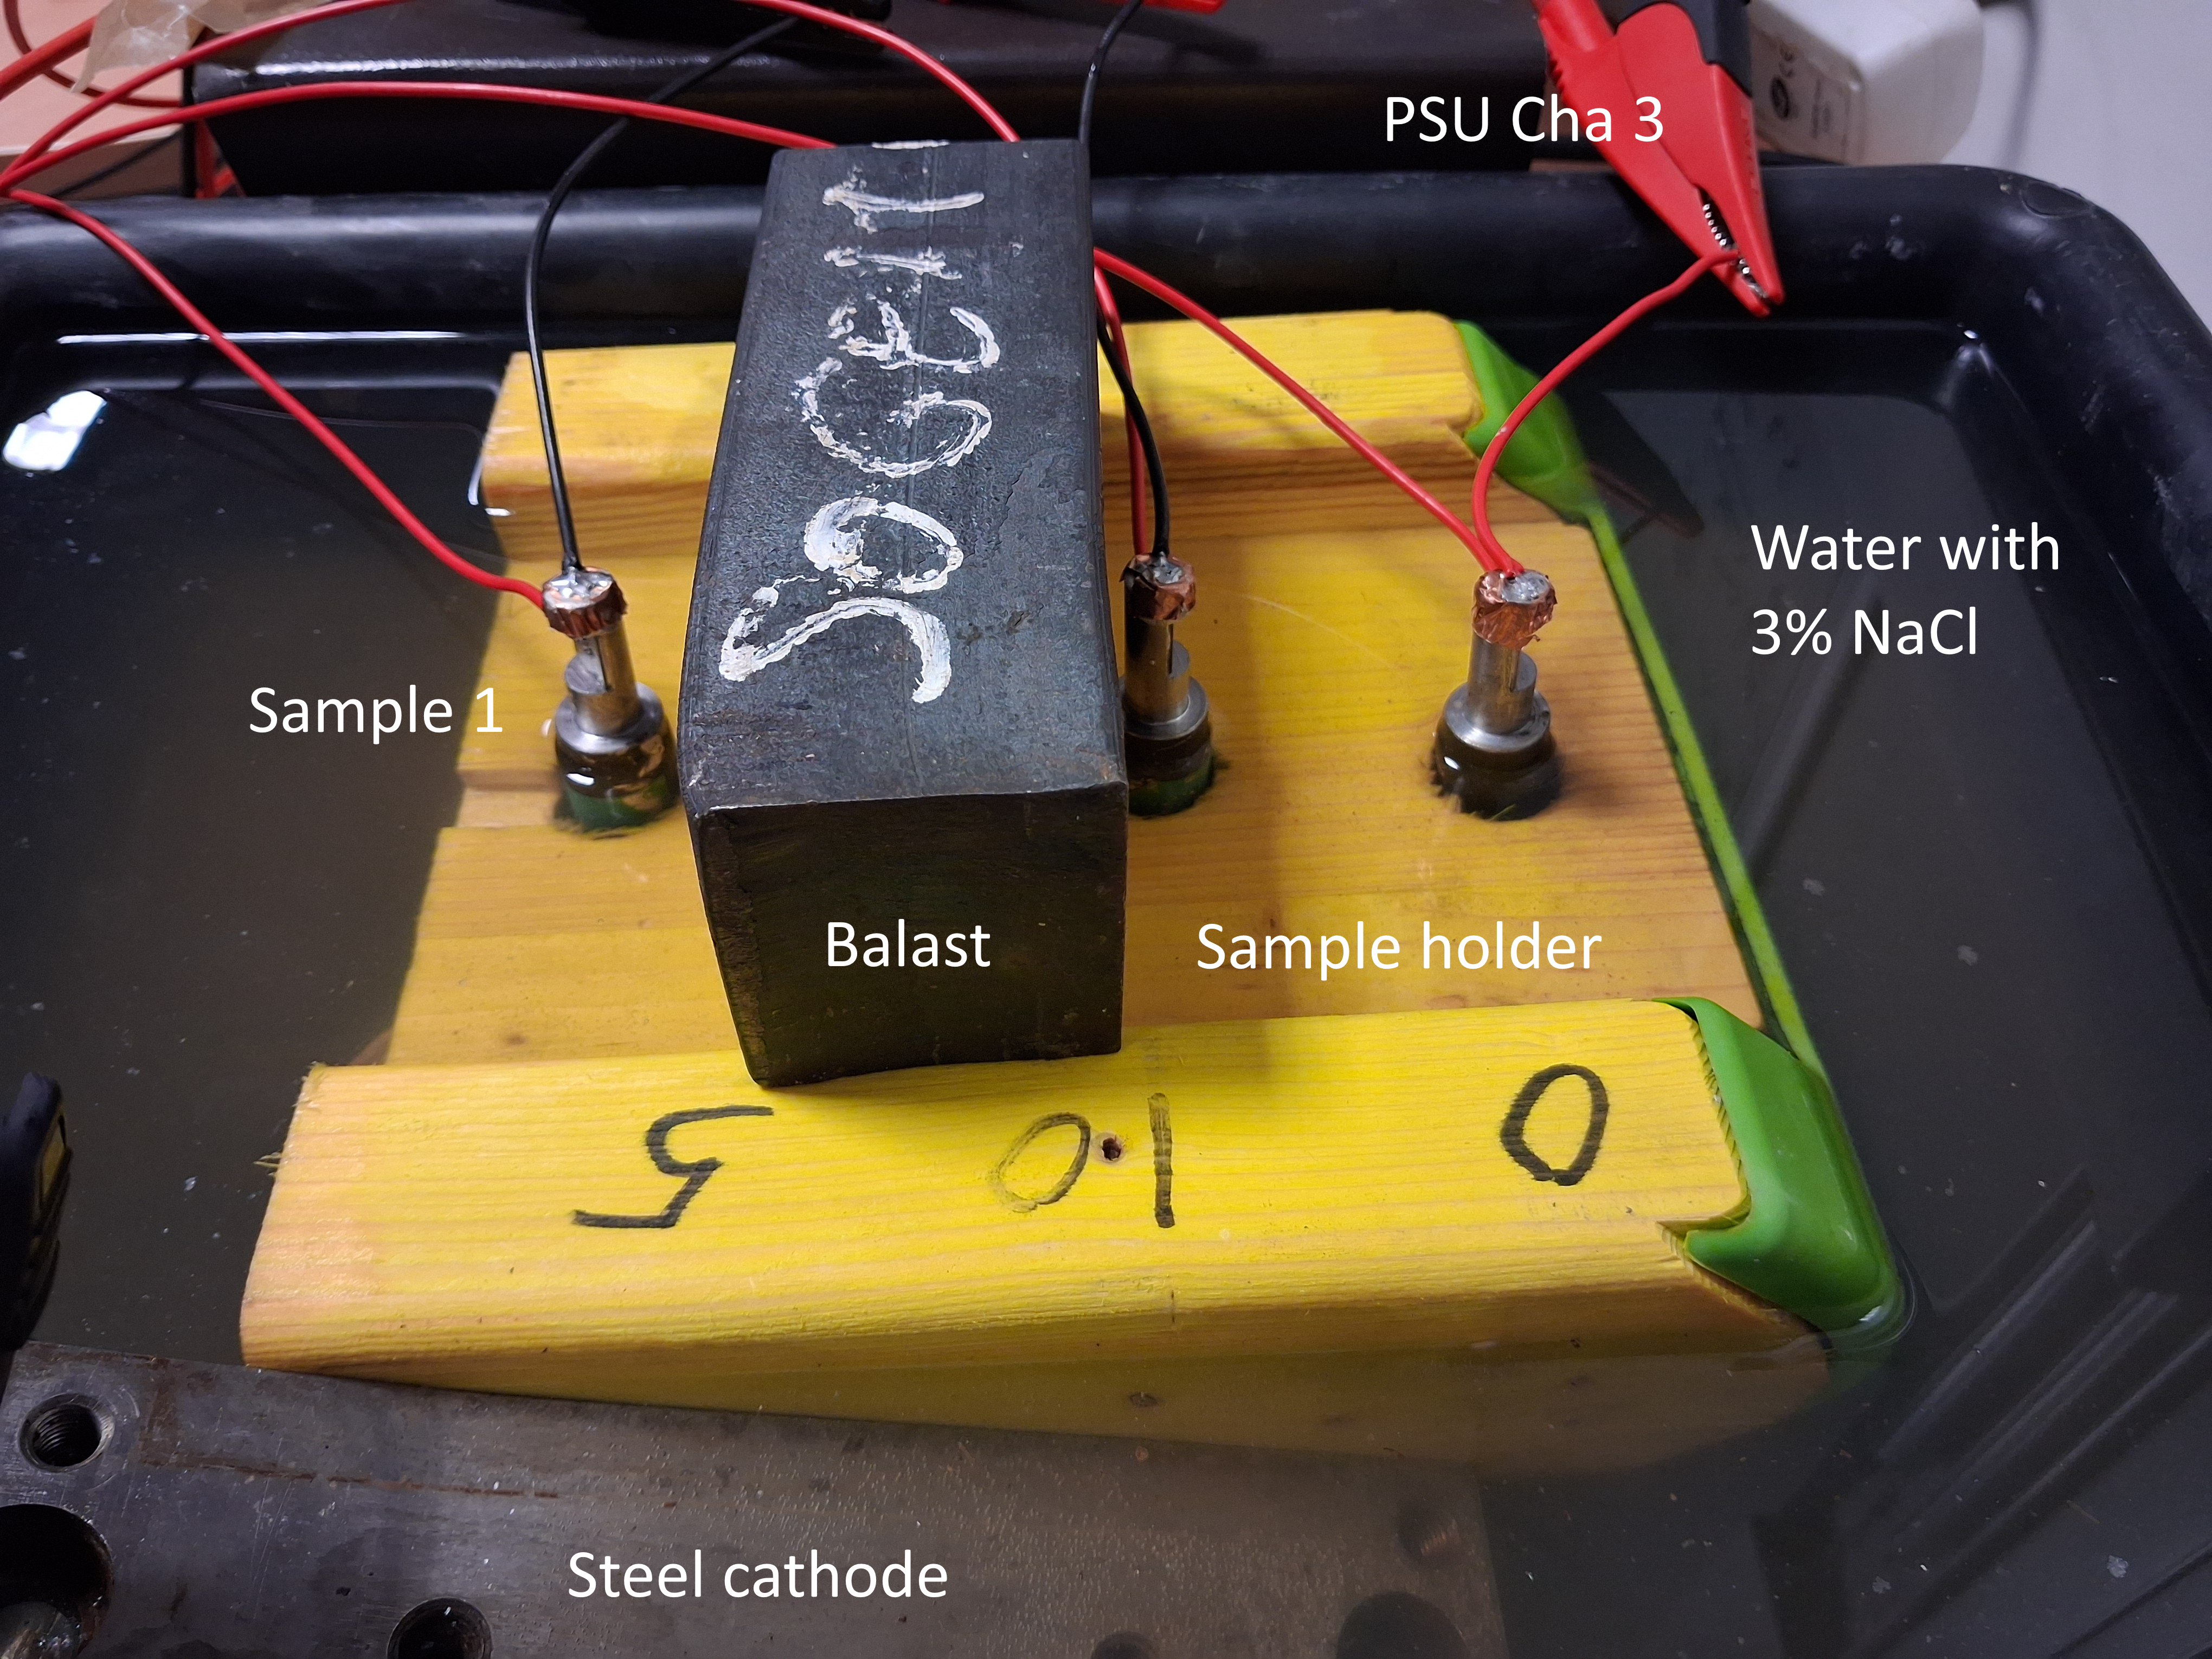
\includegraphics[width=1\linewidth]{images/Test-Setup-UTTOP-Annotated.png}
    \caption{Samples submerged in 3\,\% NaCl solution during the accelerated corrosion experiment. The yellow sample holder ensures the PZTs stay above the waterline. The ballast keeps the sample holder in place.}
    \label{fig:samples-in-water}
\end{figure}

\begin{comment}
    
The current through each sample over the duration of the experiment is shown in Fig.~\ref{fig:current-over-time}. Sample~1 exhibited sporadic current fluctuations; however, as shown in Fig.~\ref{fig:calibrated-mass-loss}, its cumulative mass loss remained similar to that of Samples~2 and~3, which had more stable current profiles. This indicates that the current fluctuations did not significantly affect the overall mass loss.

\begin{figure}[!t]
    \centering
    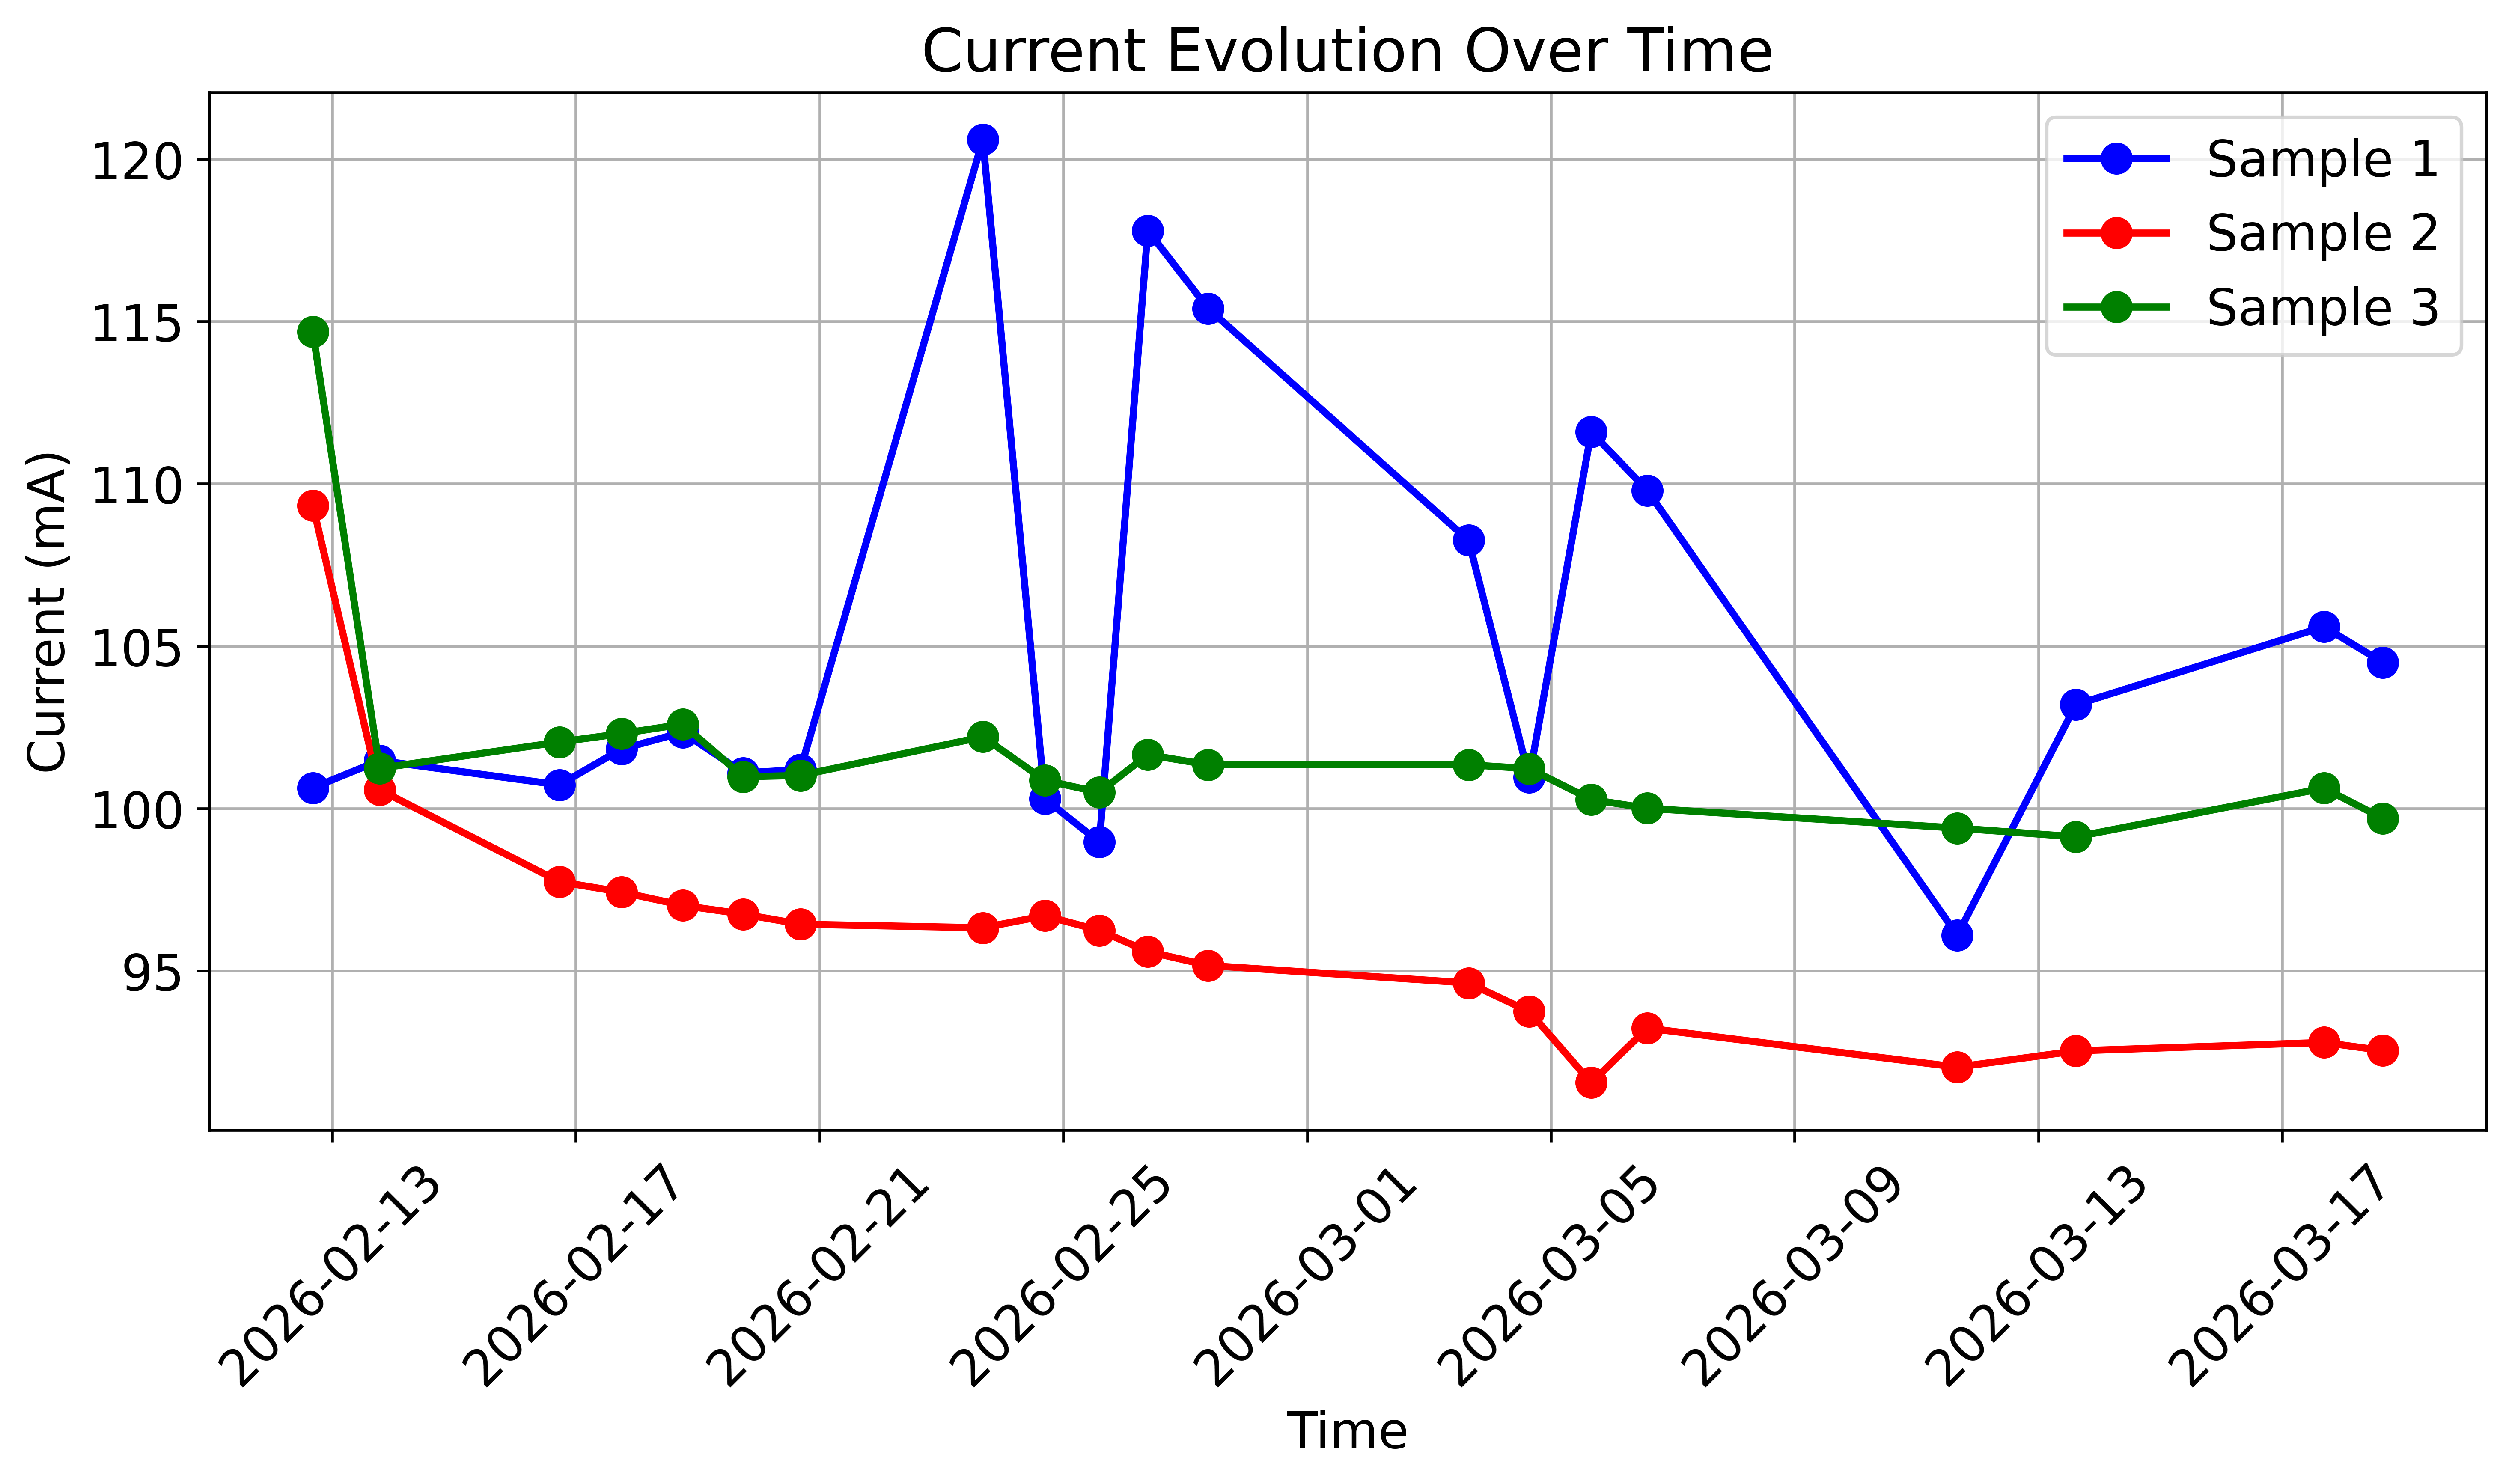
\includegraphics[width=1\linewidth]{images/current-over-time.png}
    \caption{Galvanic current measured for each sample over the duration of the experiment.}
    \label{fig:current-over-time}
\end{figure}
\end{comment}


\subsection{Mass-loss estimation}\label{sec:mass-loss}

Cumulative mass loss was estimated from the measured current using Faraday's law of electrolysis:

\begin{equation}
    \Delta m_F(t) = \sum_{j=1}^{N(t)} \frac{I_j \, \Delta t_j \, M_{\mathrm{Fe}}}{n \, F}
    \label{eq:faraday}
\end{equation}

where $I_j$ is the current (amps) through the sample measured during interval~$j$, $\Delta t_j$ is the corresponding time interval (seconds), $M_{\mathrm{Fe}} = 55.845$\,g/mol is the molar mass of iron, $n = 2$ is the number of electrons transferred per dissolved iron atom (Fe $\rightarrow$ Fe$^{2+}$), and $F = 96\,485$\,C/mol is Faraday's constant.

Because Faraday's law assumes ideal current efficiency, the estimated $\Delta m_F(t)$ can deviate from the true mass loss. To account for this, samples were periodically removed and weighed, providing ground-truth mass-loss values $m_k^{\mathrm{meas}}$ at discrete times $t_k$, $k = 0, 1, \dots, K$. A piecewise-linear calibration was then applied within each interval $t \in [t_k,\, t_{k+1}]$:

\begin{equation}
    \begin{split}
    \hat{m}(t) &= m_k^{\mathrm{meas}}
      + \frac{\Delta m_F(t) - \Delta m_F(t_k)}
             {\Delta m_F(t_{k+1}) - \Delta m_F(t_k)}
        \left( m_{k+1}^{\mathrm{meas}} - m_k^{\mathrm{meas}} \right)
    \end{split}
    \label{eq:piecewise_cal}
\end{equation}

This rescales the Faraday-derived curve so that $\hat{m}(t_k) = m_k^{\mathrm{meas}}$ at every weighing date while preserving the temporal shape of the electrochemically derived trajectory between anchor points. 

%The calibrated mass-loss curves are shown in Fig.~\ref{fig:calibrated-mass-loss}.

%\begin{figure}[!t]
%    \centering
%    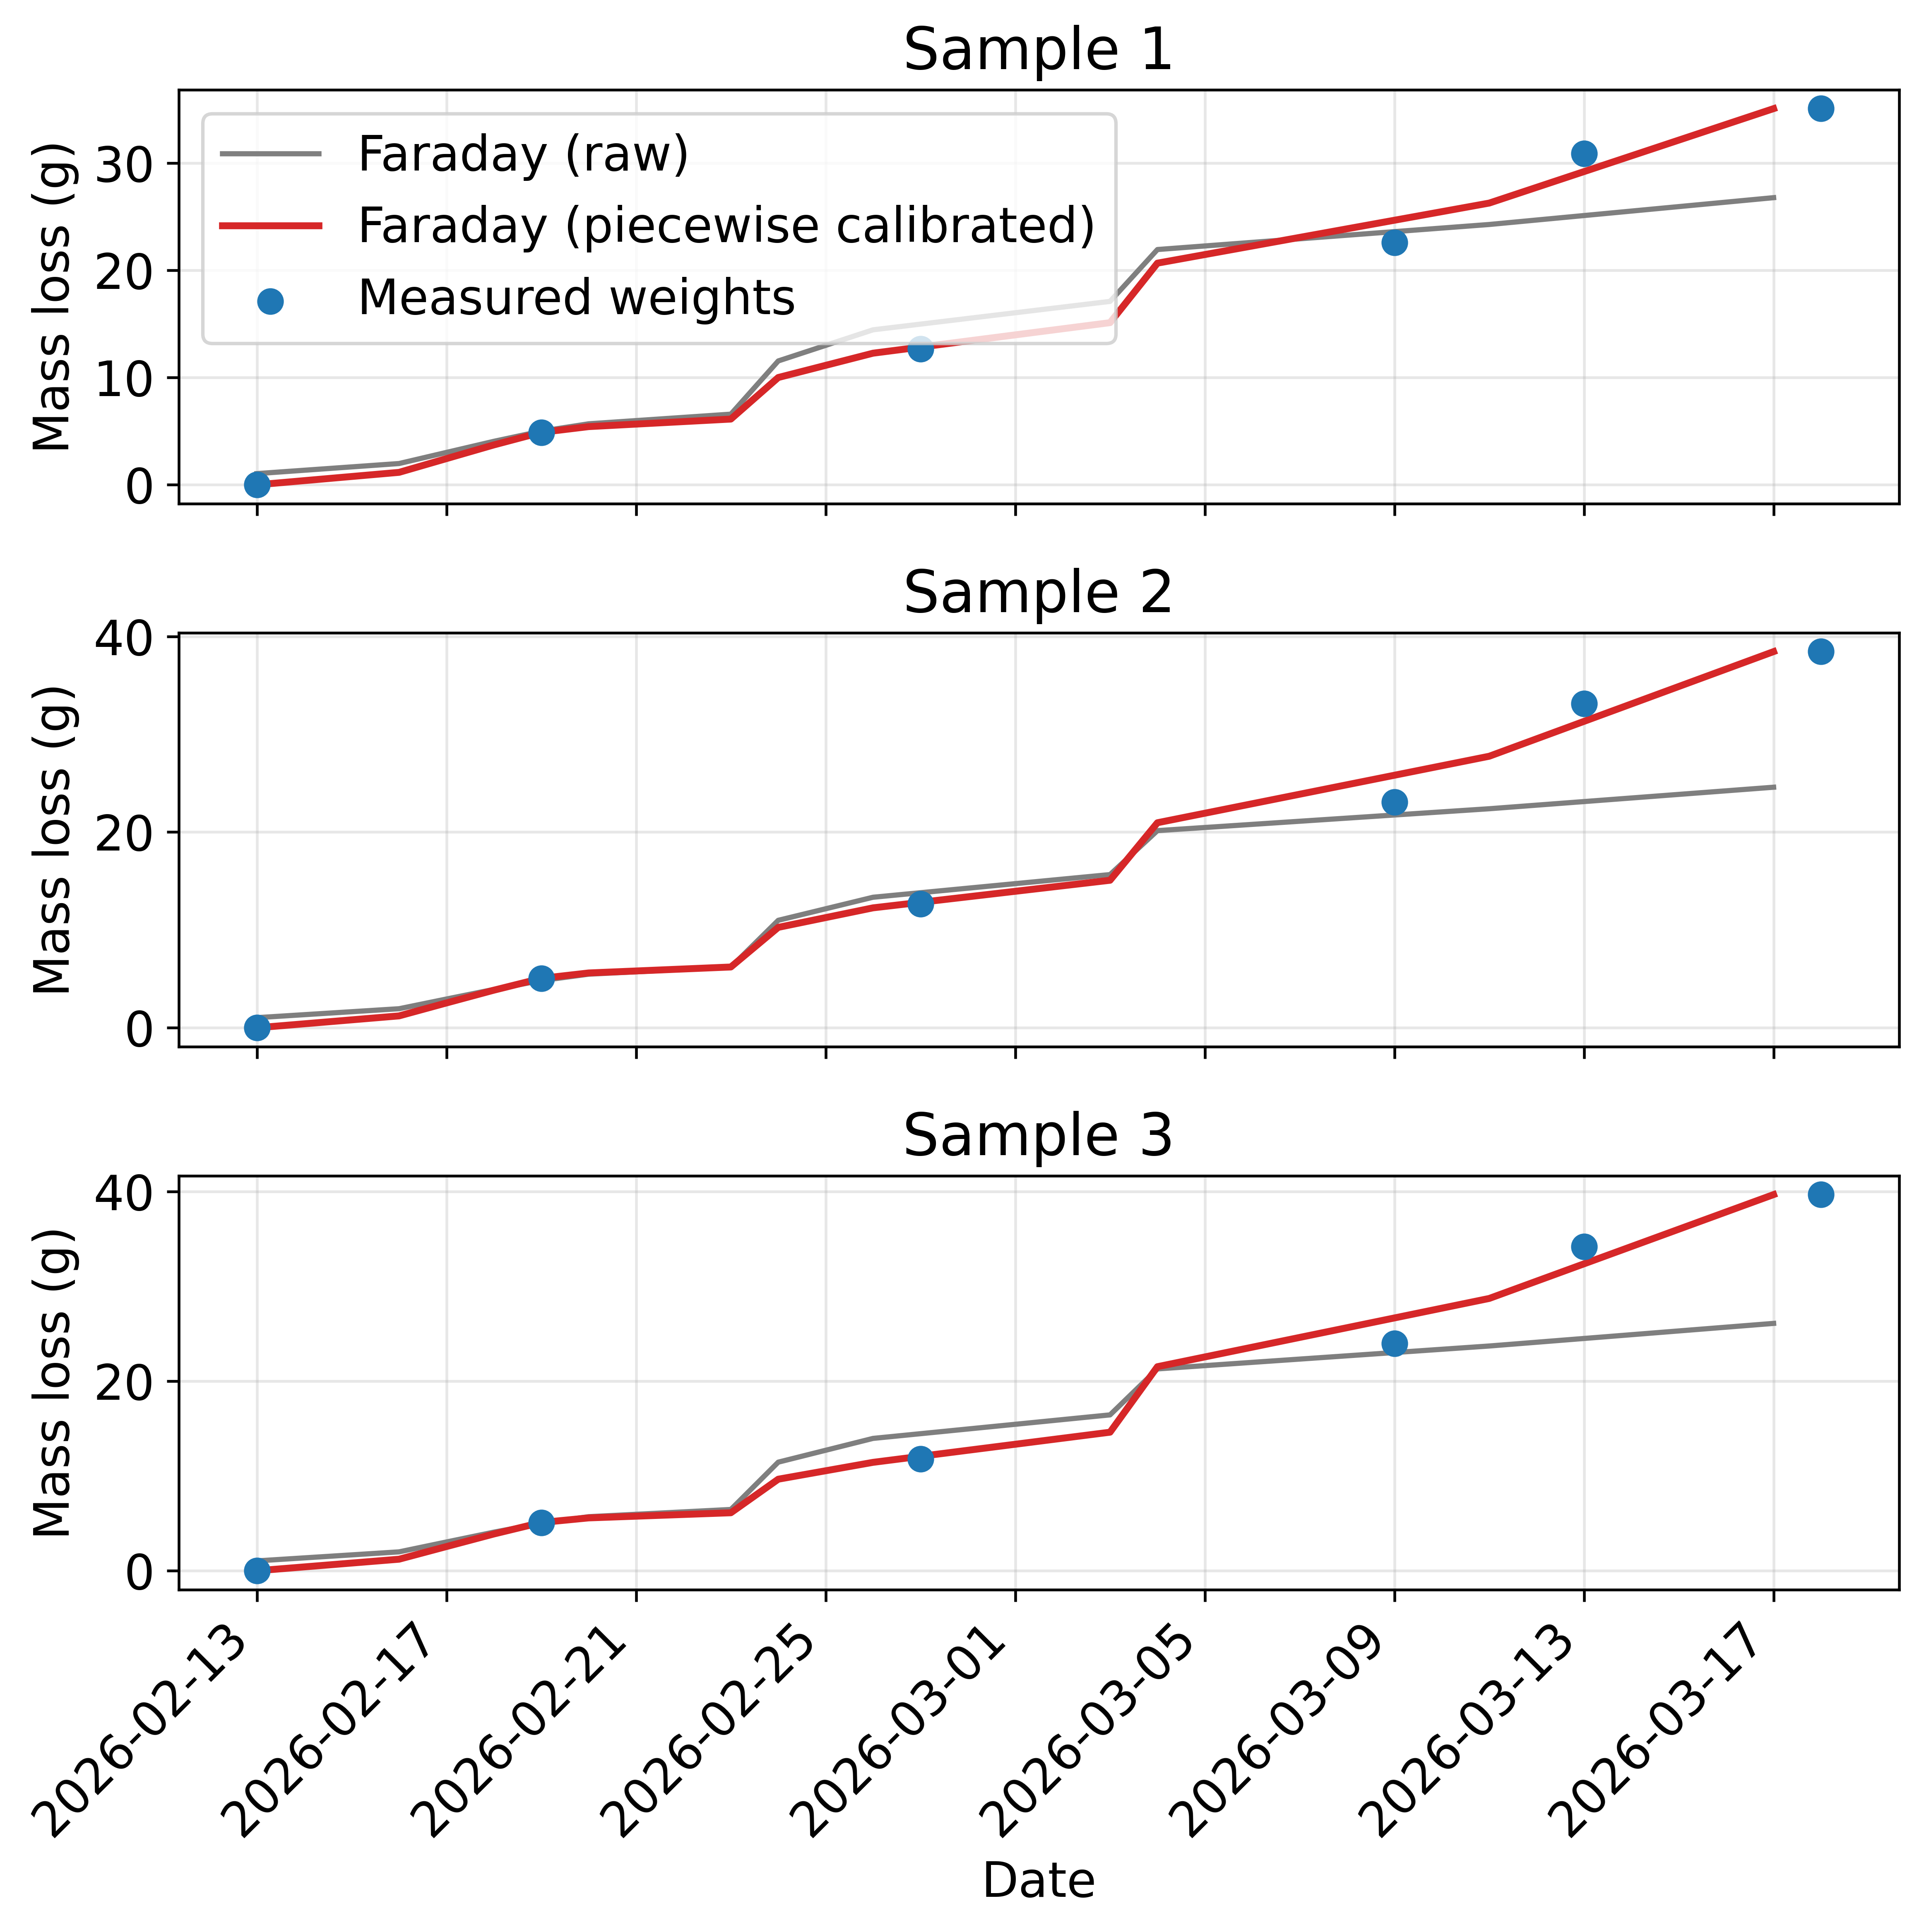
\includegraphics[width=0.75\linewidth]{images/Calibrated-mass-loss.png}
%    \caption{Faraday-derived mass loss before and after piecewise-linear calibration against %measured mass-loss values.}
%    \label{fig:calibrated-mass-loss}
%\end{figure}


\subsection{BVD feature extraction}\label{sec:feature-engineering}

As described in Section~\ref{sec:introduction}, the BVD equivalent circuit is fitted to the real part of each measured impedance signature to extract five circuit parameters ($R_0$, $R_1$, $L_1$, $C_1$, $C_0$). Since the BVD circuit models a single resonance peak, the impedance data are restricted to the frequency region containing the dominant resonance observed across all three samples (see Fig.~\ref{fig:RMSD-peaks}). This ensures consistent parameter extraction while focusing on the most informative part of the signal.

The fitting is performed using the differential evolution optimizer from the SciPy library \cite{diff-evolution}, which minimizes the RMSD between the measured and modeled real impedance.

%\begin{equation}
%\min_{(R_0, R_1, L_1, C_1, C_0)} ; \mathrm{RMSD}\left(\mathrm{Re}{Z_{\mathrm{meas}}},; \mathrm{Re}{Z_{\mathrm{BVD}}}\right)
%\label{eq:BVD-fit}
%\end{equation}

To incorporate prior physical knowledge, constraints are imposed during the optimization. The parameter $L_1$ is initialized to $20$ mH to reflect a known initial effective mass, and is further constrained to decrease monotonically across successive measurements during the fitting process, this captures the expected reduction in mass due to progressive corrosion. As several combinations of BVD parameters can yield a similar impedance, the fitting also includes an added penalty for changing $L_1$, the algorithm will thus prioritize adjusting the 4 remaining parameters anchoring the fitting around $L_1$ or the mass loss. Additionally, all parameters ($R_0$, $R_1$, $L_1$, $C_1$, $C_0$) are constrained to be non-negative to ensure physically meaningful solutions.

The complete processing pipeline is as follows: First, the real part of the impedance is measured over time, $\mathrm{Re}(Z, t)$. The BVD parameters are then obtained by minimizing the deviation between the measured impedance and the model response. Finally, the extracted parameters are normalized relative to their initial (reference) values using the scaling defined in Eq.~\ref{eq:rel-scaler}, producing the feature vector [$\mathrm{rel}_{R0}$, $\mathrm{rel}_{R1}$, $\mathrm{rel}_{L1}$, $\mathrm{rel}_{C1}$, $\mathrm{rel}_{C0}$] used as input to the neural network.

This BVD-based fitting procedure serves as a feature extraction step that reduces the high-dimensional impedance signal to a compact, physically interpretable representation. By focusing on the evolution of the dominant resonance, it mitigates sample-specific variations while preserving the information relevant to structural degradation. The temporal evolution of the fitted parameters for each sample is shown in Fig.~\ref{fig:BVD-param-over-time}.

\begin{comment}
    
\begin{figure}[!t]
    \centering
    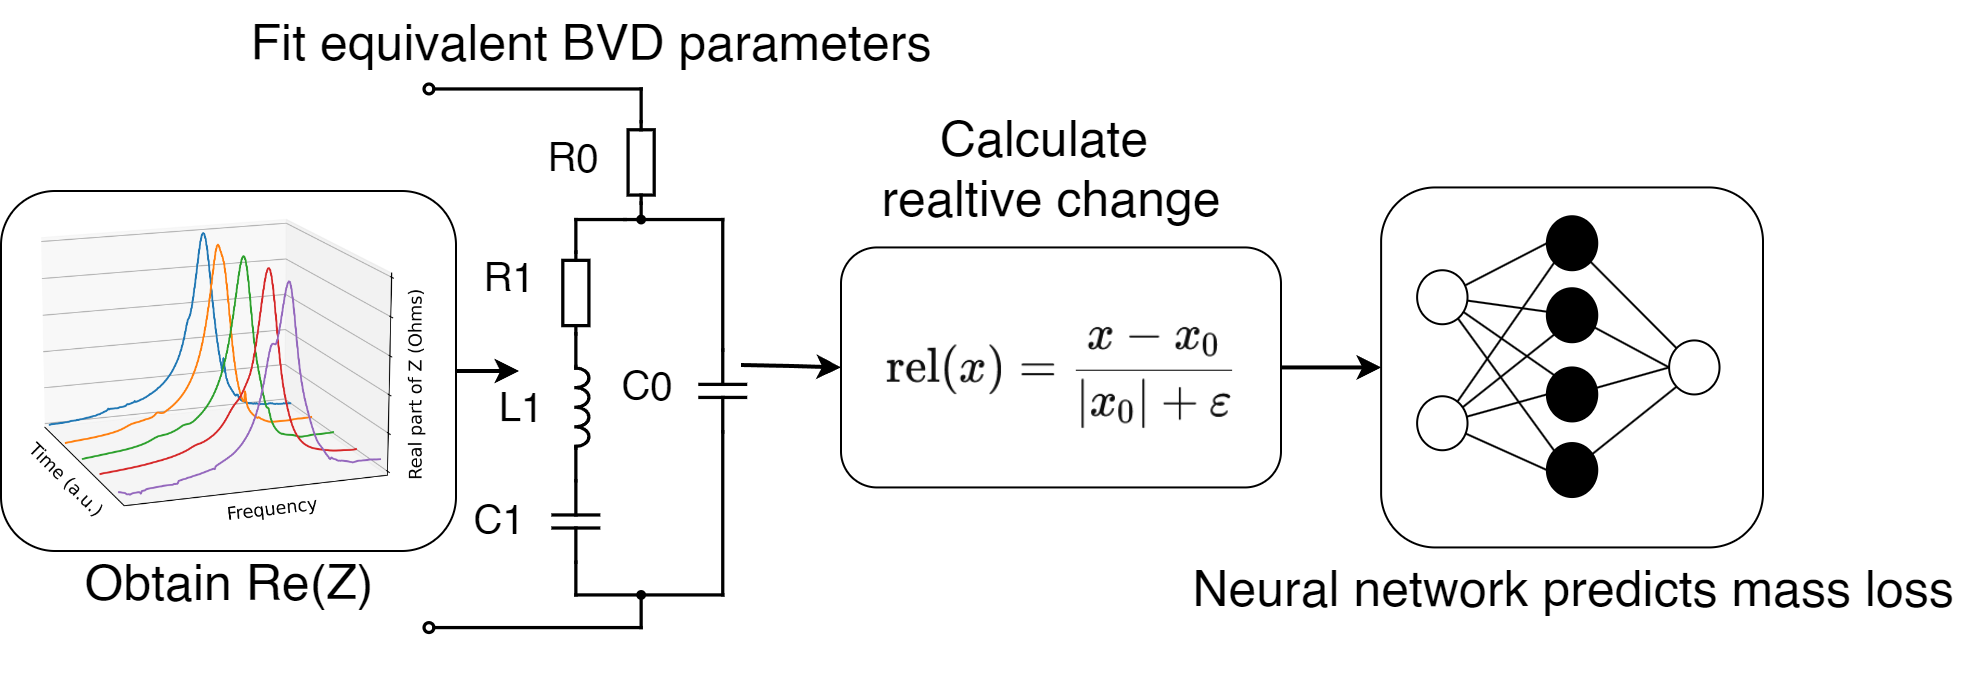
\includegraphics[width=1\linewidth]{images/UTTOP_MLV2.drawio.png}
    \caption{Full pipeline: impedance data is acquired over time, BVD parameters are extracted via constrained fitting, and their relative changes are used as input features for neural network mass-loss prediction.}
    \label{fig:ML-diagram}
\end{figure}

\end{comment}


\subsection{Model architectures}\label{sec:models}

Two Convolutional Neural Networks (CNNs) regression models were compared for predicting mass loss from impedance-derived features. The models enforce non-negative outputs using a Softplus activation in the final layer, $\hat{y} = \ln(1 + e^z)$, where $z$ is the pre-activation output.

Data augmentation was applied prior to training increasing the size of the dataset by 20 times using samples generated through interpolation, a small Gaussian noise with a standard deviation of 5\% of each feature’s standard deviation was added to the relative impedance features. This increases the effective dataset size while introducing controlled variability.

All models were trained using the Adam optimizer with mean squared error (MSE) loss, and early stopping based on validation loss was employed to prevent overfitting.

Generalization performance was evaluated using LOO cross-validation. In each fold, one of the three samples was held out as the test set, while the remaining two samples were used for training. This procedure directly evaluates the model’s ability to predict mass loss on a previously unseen sample.

A small grid search over the hyperparameters listed in Table~\ref{tab:hyperparams} was performed for each model.

\begin{table}[ht]
\centering
\small
\begin{tabular}{llc}
\hline
\textbf{Model} & \textbf{Hyperparameter} & \textbf{Values Searched} \\
\hline
1D-CNN
 & Learning Rate        & \{1e-1, 1e-2, 1e-3, 1e-4\} \\
 & Weight Decay         & \{0, 1e-4, 1e-3, 1e-2, 1e-1\} \\
 & Scaler               & \{standard, power, quantile\} \\
 & Number of Filters    & \{8, 16, 32, 64\} \\
 & Kernel Size          & \{1, 2, 3, 4, 5\} \\
 & Conv Layers          & \{1, 2, 3, 5\} \\
 & Dropout              & \{0.0, 0.01, 0.05, 0.1\} \\
 & Window Size          & \{3, 5, 7\} \\
\hline

\end{tabular}
\caption{Hyperparameters and values searched during grid search for the 1D-CNN models.}
\label{tab:hyperparams}
\end{table}

\subsubsection{Raw impedance model}

A 1D CNN model were trained on the unprocessed (“raw”) impedance data, where the input consists of the real part of the impedance around the main peak seen in Fig.~\ref{fig:RMSD-peaks}, resulting in a 1400-dimensional feature vector.

The input was standardized to zero mean and unit variance using:

\begin{equation}
x_{\mathrm{scaled}} = \frac{x - \mu}{\sigma}
\end{equation}

where $\mu$ and $\sigma$ are computed from the training set.

The best performing CNN model used two convolutional blocks (16 and 32 filters, kernel size 5), each followed by batch normalization, ReLU activation, and dropout. A global average pooling layer reduced the feature dimension, followed by a fully connected head (16 neurons) and a Softplus output neuron.

\subsubsection{BVD-informed neural network}

Another 1D-CNN model were trained using the five parameters extracted from the Butterworth–Van Dyke (BVD) model (Section~\ref{sec:feature-engineering}).

The features were normalized using relative scaling:

\begin{equation} 
    x_{\mathrm{rel},i} = \frac{x_i - x_{0}}{|x_{0}| + \epsilon} 
    \label{eq:rel-scaler}
\end{equation}

where $x_i$ is the feature value at the $i$-th measurement, $x_0$ is the corresponding value from the reference measurement, and $\epsilon = 10^{-30}$ prevents division by zero. This normalization emphasizes changes relative to the baseline state, enhancing sensitivity to damage progression.

The best performing CNN model used the same architecture as in the raw impedance case, but adapted to the 5-dimensional input. Specifically, two convolutional layers (16 and 32 filters, kernel size 5) were applied, followed by batch normalization, ReLU activation, and dropout. The resulting features were aggregated using global average pooling and passed through a small fully connected head (16 neurons) with a Softplus output.


\begin{comment}
    

\subsubsection{Polynomial model}

The polynomial model augments the input feature space with element-wise polynomial expansions up to degree $d$. For an input vector $\mathbf{x} \in \mathbb{R}^{n}$, the expanded feature vector is:

\begin{equation}
    \phi(\mathbf{x}) = \left[\mathbf{x},; \mathbf{x}^{\circ 2},; \dots,; \mathbf{x}^{\circ d} \right]
\end{equation}

where $\mathbf{x}^{\circ k}$ denotes element-wise exponentiation. This approach is included to evaluate whether non-linear relationships in the data can be captured through a simple feature expansion, without relying on the representational complexity of a neural network. As such, the polynomial model serves as a baseline for assessing whether a more complex model is necessary, or if comparable performance can be achieved with a simpler formulation.

The model coefficients are optimized using the Adam optimizer with mean squared error (MSE) loss, consistent with the training procedure used for the BVD-based neural network. Several polynomial degrees were evaluated, with the best-performing configuration obtained for $d=3$.

\end{comment}


\section{Results}\label{sec3}

This section first evaluates the conventional RMSD metric for damage tracking, then compares the machine learning models under LOO cross-validation as discussed in Section~\ref{sec2}.

The mass loss of Samples~1, 2, and 3 was approximately 35\,g, 38\,g, and 39\,g, respectively. Sample~1 at the start and end of the test can be seen in Fig.~\ref{fig:samples-over-time}.

\begin{figure}[!t]
    \centering
    \includegraphics[width=0.8\linewidth]{images/SamplesOverTimeAnnotated.png}
    \caption{Visual progression of corrosion on sample 1 over the duration of the experiment. The orange arrow indicates the location of the PZT patch.}
    \label{fig:samples-over-time}
\end{figure}


\subsection{RMSD analysis}

The RMSD (Eq.~\ref{eq:rmsd}) was computed over the main resonant peak of the real part of the impedance signature, in the frequency range shown in Fig.~\ref{fig:RMSD-peaks}.

\begin{figure}[!t]
    \centering
    \includegraphics[width=1\linewidth]{images/RMSD-peak.png}
    \caption{Real part of the impedance form the first and last measurement of each sample, limited to the frequency range around the main resonance peak used for RMSD computation.}
    \label{fig:RMSD-peaks}
\end{figure}

Fig.\ref{fig:RMSD-score} shows the RMSD score for each sample plotted alongside the calibrated mass loss over time. While the RMSD generally increases with damage, it does not increase monotonically: the curves fluctuate substantially and, at several points, different mass-loss levels produce similar RMSD values. The RMSD is particularly unreliable at low damage levels, where it struggles to distinguish early-stage corrosion, and even at higher damage levels it is possible for a given mass-loss state to yield a misleadingly low score. For example, the RMSD of Sample 1 at approximately 12g of mass loss is comparable to its value at 35g, despite a significant difference in actual damage. Under the studied conditions, the RMSD alone is therefore insufficient as a standalone metric for quantitative damage tracking.


\begin{figure}[!t]
    \centering
    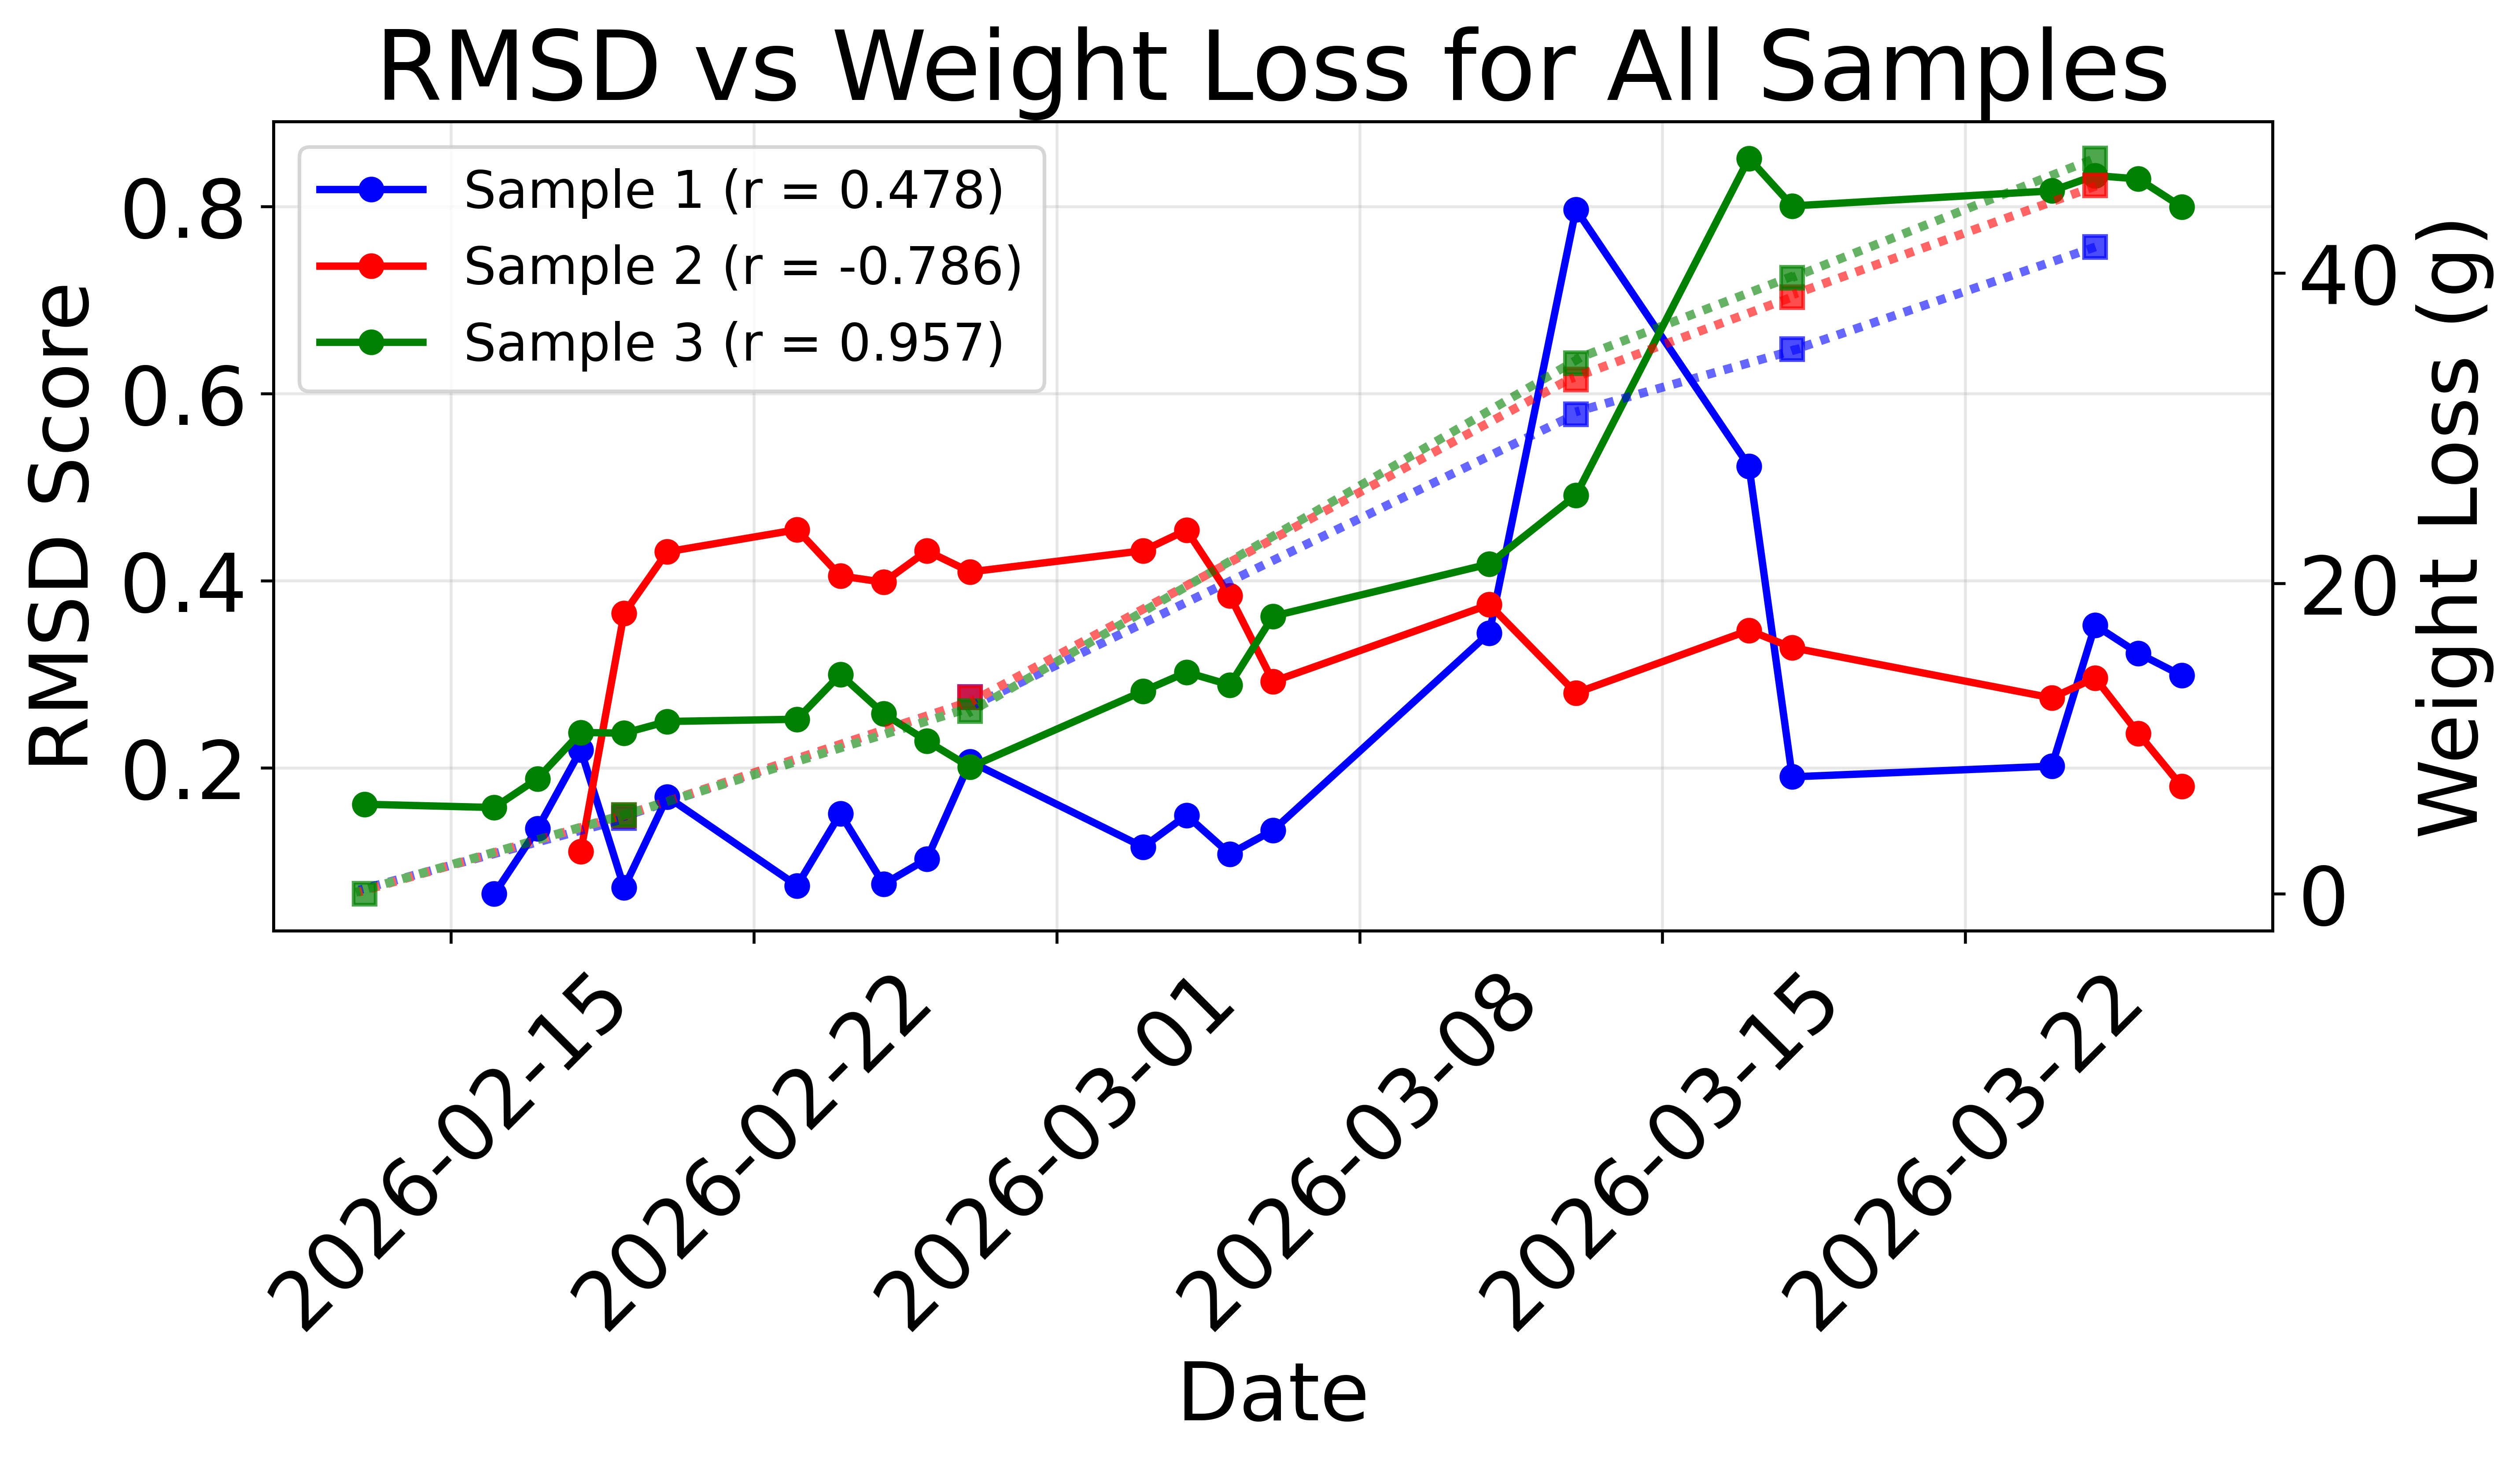
\includegraphics[width=0.85\linewidth]{images/RMSD-Score.png}
    \caption{RMSD score (left axis) and calibrated mass loss (right axis) over time for each sample. The non-monotonic RMSD evolution illustrates the limitations of RMSD for quantitative damage tracking. The dashed lines indicate the mass loss of each sample.}
    \label{fig:RMSD-score}
\end{figure}

\subsection{Environmental factors}

The air temperature and relative humidity (\%RH) were recorded at the time of each impedance measurement, both remained relatively stable throughout the experiment, with temperature ranging from approximately 20--27\,°C and humidity from 30--51\,\%RH. Given this stability and the low sampling frequency, temperature and humidity were excluded as input features in subsequent analyses.

\begin{comment}
    
\begin{figure}[h]
    \centering
    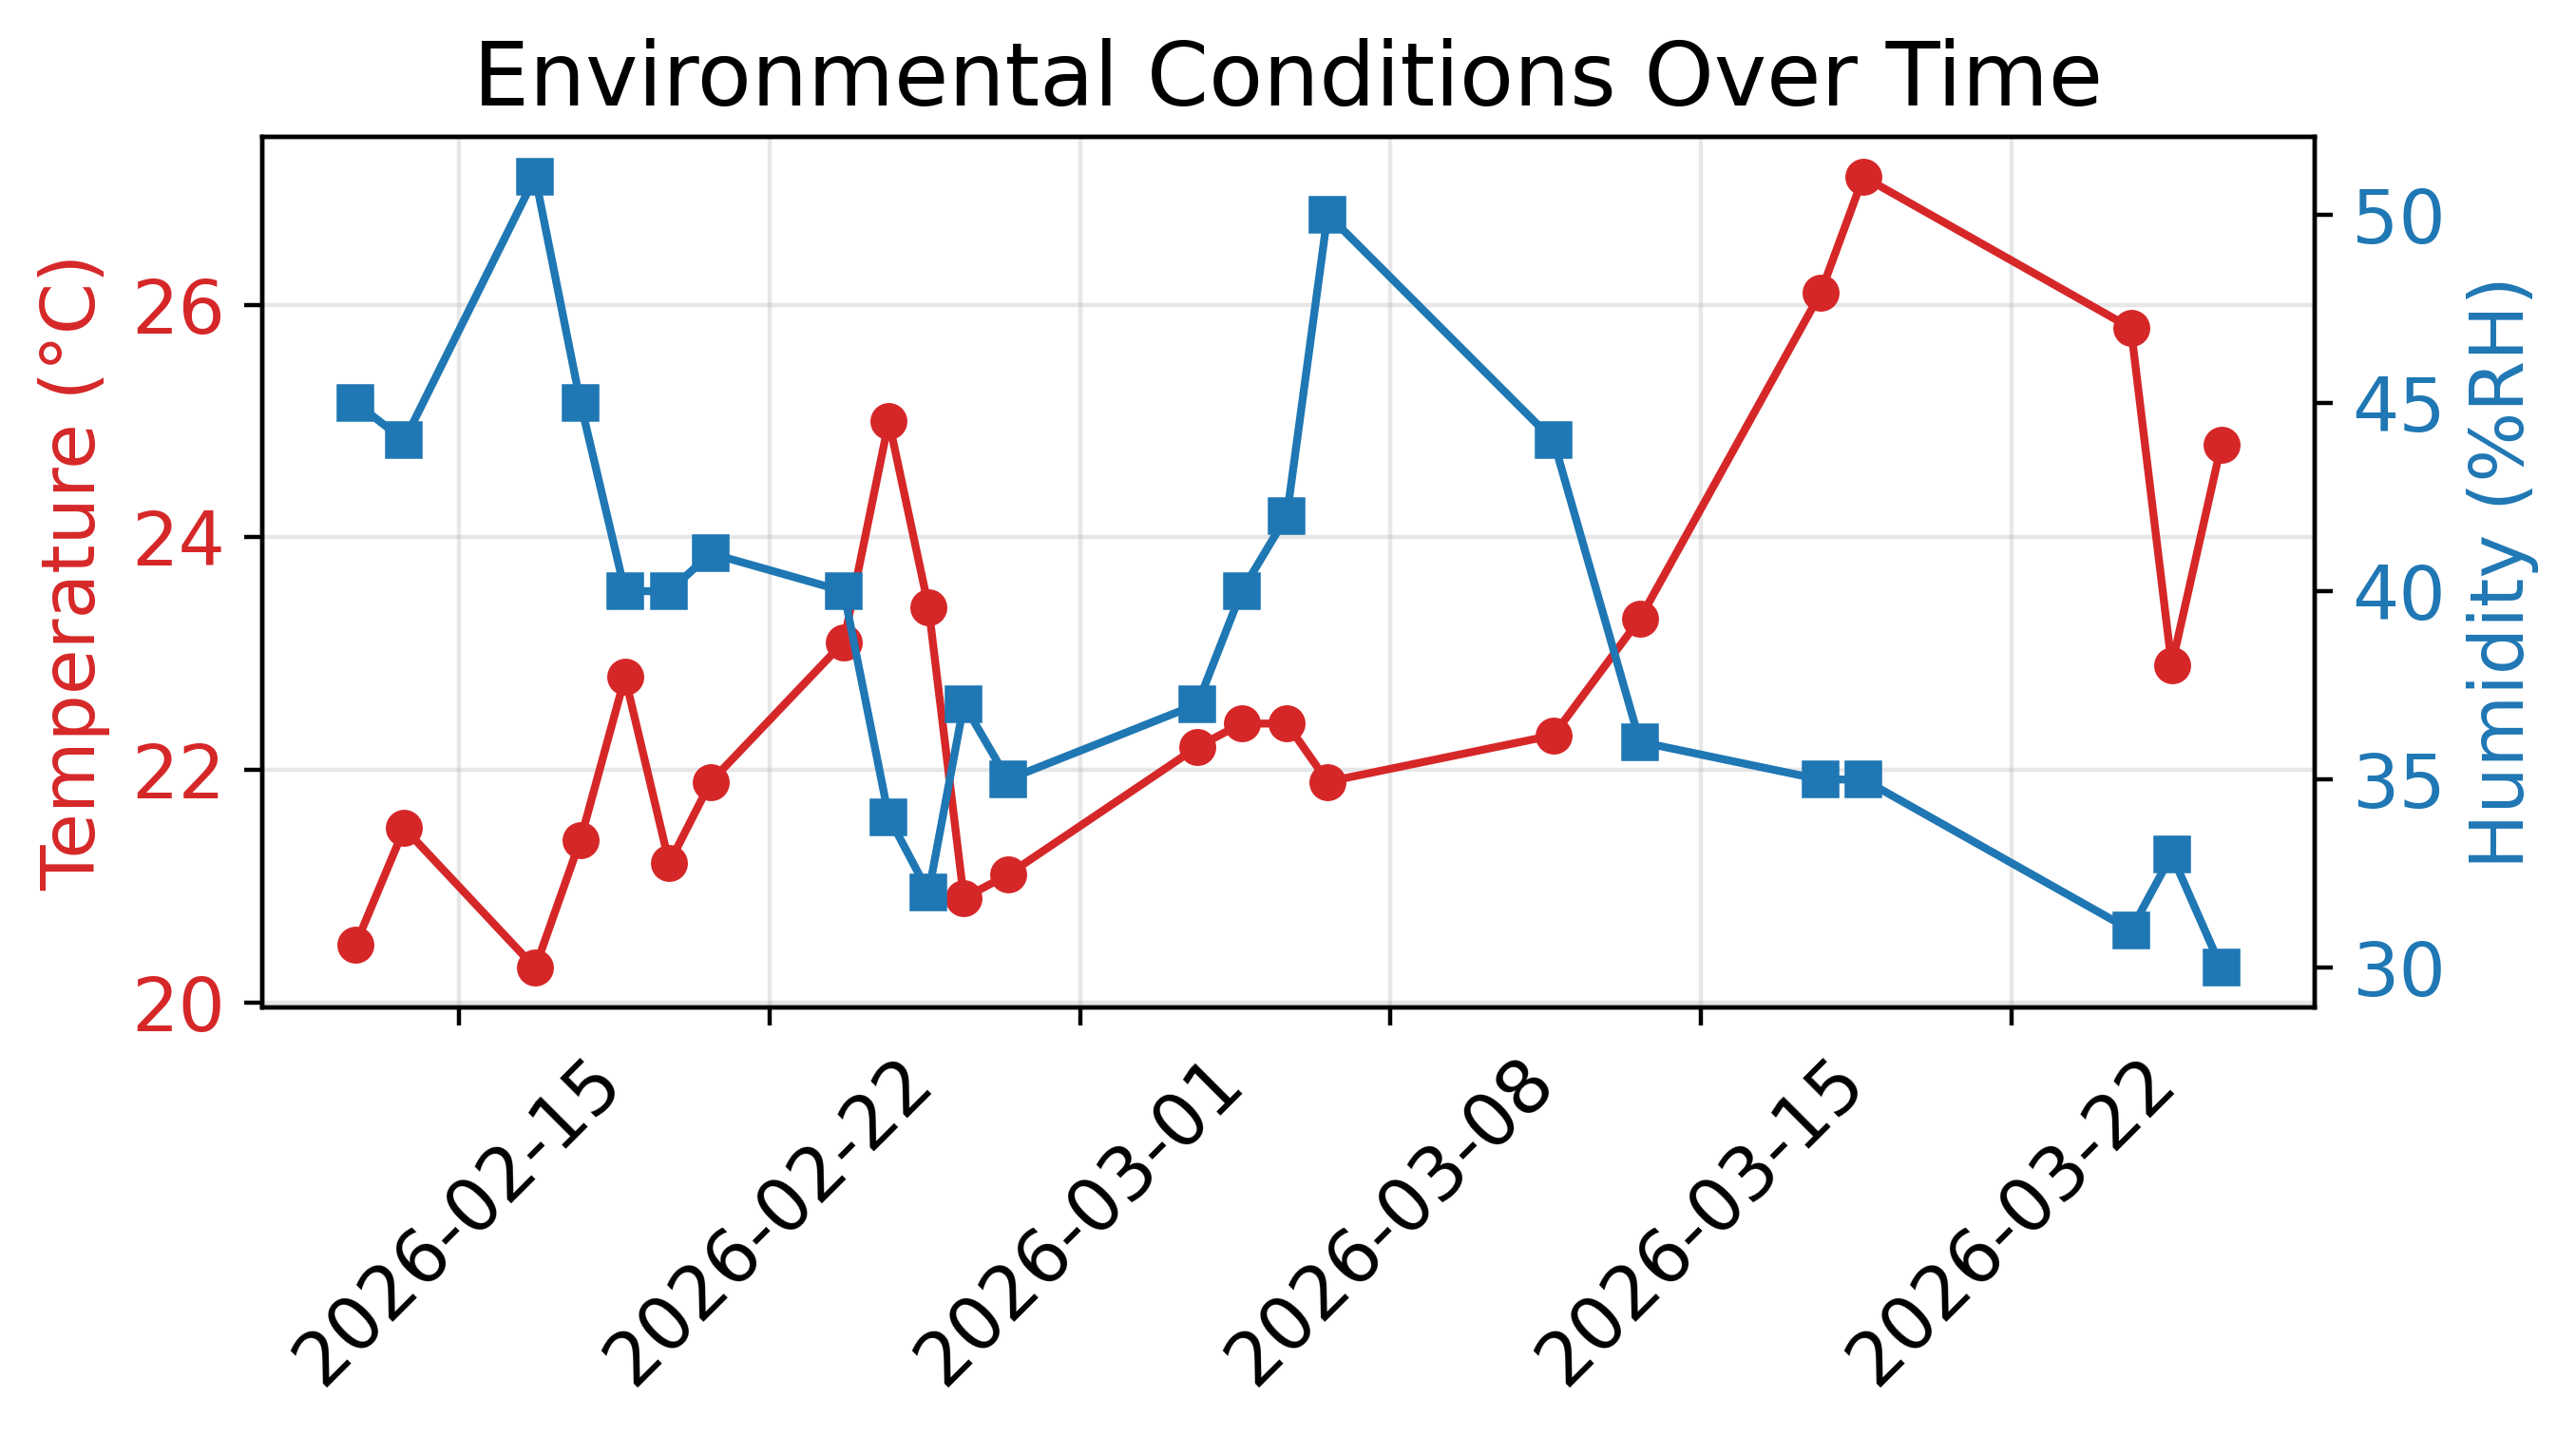
\includegraphics[width=1\linewidth]{images/Temp-RH-over-time.png}
    \caption{Air temperature and relative humidity (\%RH) recorded at the time of each impedance measurement.}
    \label{fig:temp-rh-over-time}
\end{figure}

\end{comment}


\subsection{BVD feature extraction}

Fig.~\ref{fig:BVD-param-over-time} shows the evolution of the fitted BVD parameters, the resonant frequency, the Q-factor, and the fitting quality ($\mathrm{R}^2$) over time for each sample. The motional inductance $L_1$ decreases consistently across all three samples, reflecting the progressive mass loss due to corrosion. The motional resistance $R_1$ and capacitance $C_1$ also exhibit clear trends. The static capacitance $C_0$ and series resistance $R_0$ remain relatively stable, as expected since these parameters are primarily determined by the PZT patch and bonding layer rather than the structural mass. The average fitting quality described by $R^2$ was $\approx0.85$, capturing most of the changes in the resonant peak frequency, amplitude and Q factor, but less so the details of the peaks as seen in fig \ref{fig:RMSD-peaks}.

\begin{figure}[!t]
    \centering
    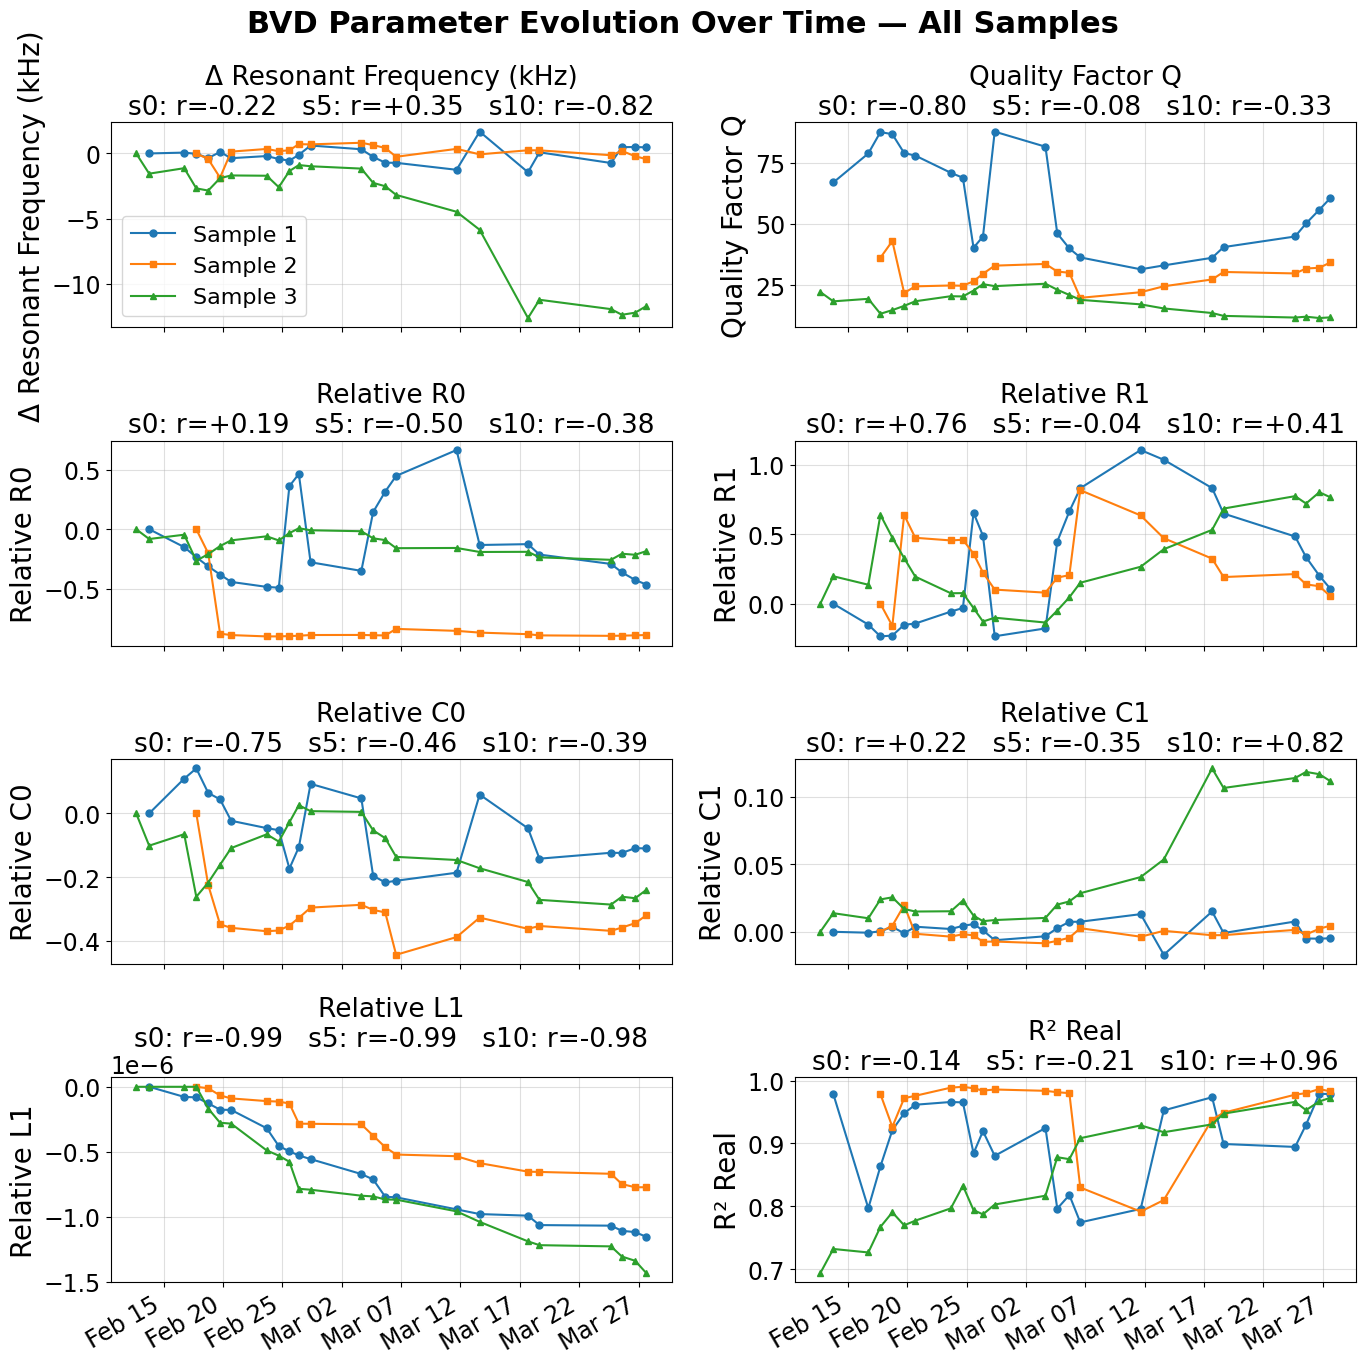
\includegraphics[width=1\linewidth]{images/BVD_Param_over_time.png}
    \caption{Evolution of the change in resonant frequency, Q-factor, fitted BVD parameters ($R_0$, $R_1$, $L_1$, $C_1$, $C_0$) as well as the fitting quality between the experimental data and the BVD circuit model $\mathrm{R}^2$ over time for each sample.}
    \label{fig:BVD-param-over-time}
\end{figure}

\subsection{Machine learning performance}

The four models described in Section~\ref{sec:models} were evaluated using LOO cross-validation. In each fold, the model was trained on two samples and tested on the held-out third sample; the reported metrics are aggregated across all three folds, table~\ref{tab:model_results} summarizes the results from all evaluated models.


\begin{table*}[!t]
\centering
\caption{Performance comparison of the 1D-CNN models using full dataset and BVD features.}
\label{tab:model_results}
\renewcommand{\arraystretch}{1.15}
\setlength{\tabcolsep}{5pt}
\begin{tabular}{llcccccc}
\hline
\textbf{Dataset} & \textbf{Model} & \textbf{Hold-out} & \textbf{Tr RMSE} & \textbf{Val MAE} & \textbf{Val $R^2$} & \textbf{Val RMSE Mean $\pm$ Std} \\
\hline

Raw Impedance & 1D-CNN
& Sample 1 & 14.61 & 9.68 & 0.16 & $11.81 \pm 0.43$ \\
& & Sample 2 & 8.48  & 4.36 & 0.87 & $5.28 \pm 0.17$ \\
& & Sample 3 & 9.43  & 9.87 & 0.28 & $11.73 \pm 0.34$ \\
& & Avg.     & 10.84 & 7.97 & 0.44 & $9.61 \pm 0.31$ \\
\hline

BVD & 1D-CNN
& Sample 1 & 4.70 & 2.61 & 0.91 & $3.85 \pm 0.22$ \\
& & Sample 2 & 3.26 & 1.12 & 0.99 & $1.41 \pm 0.06$ \\
& & Sample 3 & 1.96 & 1.90 & 0.97 & $2.28 \pm 0.09$ \\
& & Avg.     & 3.31 & 1.88 & 0.96 & $2.51 \pm 0.12$ \\
\hline

\end{tabular}
\end{table*}

\begin{comment}
\begin{figure}[!t]
    \centering
    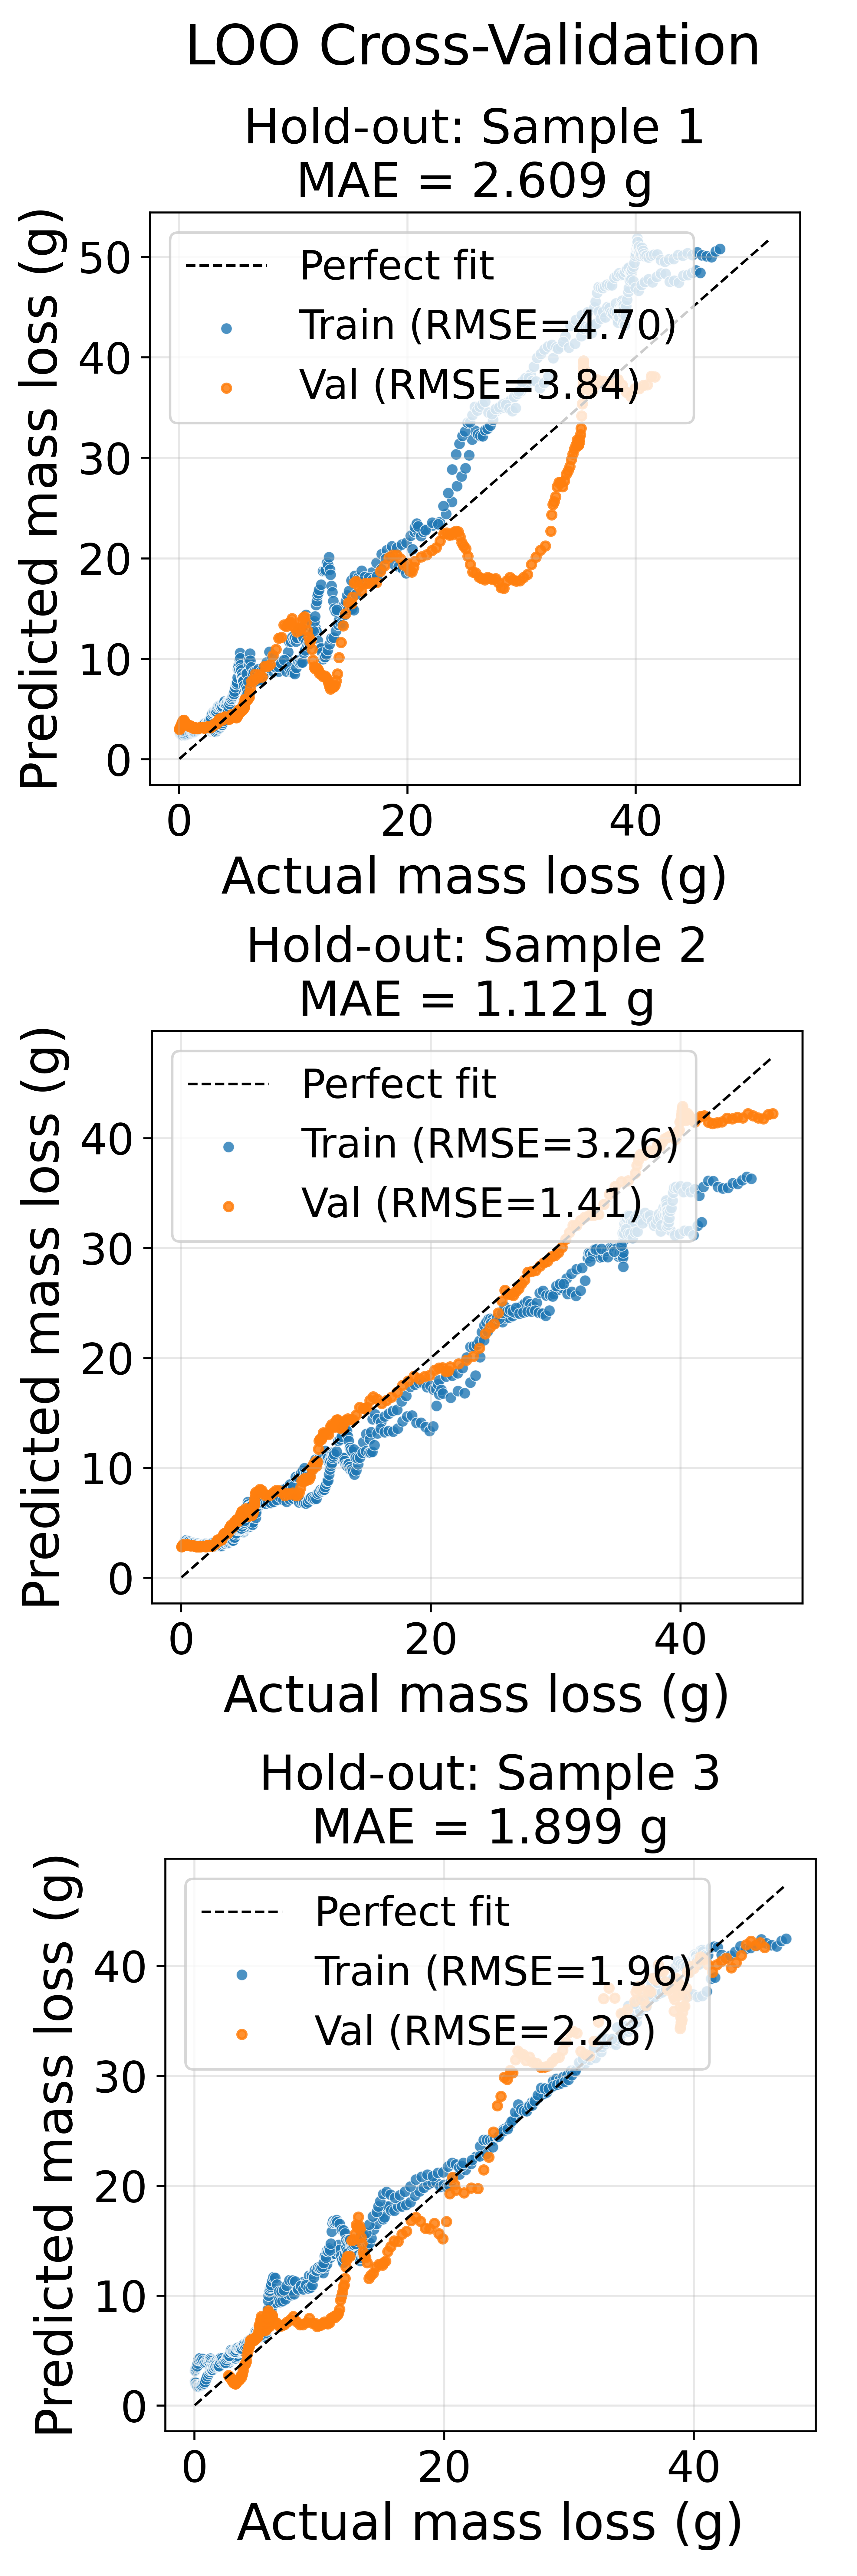
\includegraphics[width=0.55\linewidth]{images/CNN_Parity_Plots_LOO_Vert.png}
    \caption{Predicted vs.\ actual mass loss for the best performing model (1D-CNN using BVD parameters) under LOO cross-validation. Each subplot shows the predictions when the corresponding sample was held out during training.}
    \label{fig:ML-performance}
\end{figure}
\end{comment}



The model trained using the raw impedance achieved an average validation RMSE across the 3 samples of 9.61\,g. data. With the LOO validation, the model struggled to predict unseen samples, confirming that the high-dimensional impedance features are too sample-specific for cross-sample generalization.

In contrast, the BVD-informed CNN achieved substantially lower prediction errors, with an average validation RMSE across the 3 samples of 2.51\,g. This demonstrates that the BVD-feature extraction improves model generalization. 


\section{Discussion}\label{sec4}

In this section we further discuss the results from Section \ref{sec3}, focusing on interpretation, generalization, and methodological limitations.

\subsection{RMSD as a damage metric}

As shown in Section~\ref{sec3}, the RMSD is sensitive to EMI signature changes but does not provide a reliable quantitative measure of damage severity. Small amounts of damage can lead to both increases and decreases in resonant peak frequency and amplitude, making RMSD better suited for binary detection than continuous quantification of progressive damage. This motivates the use of machine learning for quantitative damage estimation.

\subsection{Generalization of impedance-based models}

LOO cross-validation shows a clear contrast between raw impedance models and BVD-based features. The raw impedance model overfit to sample-specific effects, as small variations in bonding, PZT placement, and geometry significantly affect impedance evolution.

The five BVD parameters provide a compact and physically meaningful representation that improves consistency across samples. This is further supported by the distinct impedance evolution of Sample~3 (Fig.~\ref{fig:RMSD-peaks}), which differs notably from Samples~1 and~2, yet is still well captured by the model.


\subsection{Impedance fitting}

Constraining $L_1$ to decrease monotonically improves physical consistency and prevents non-physical parameter fluctuations during fitting. This reflects the prior that corrosion reduces effective mass over time.

The differential evolution loss function attempted to minimize the RMSD between the real part of the resonant peak of the EMI data and the real part of the BVD circuit, the loss function was further penalized for changing $L_1$ to further constrain the fitting around the $L_1$ baseline.

\subsection{Application}

The primary application of this work is targeting sacrificial EMI-based sensor probes for use in reinforced concrete corrosion monitoring. Future research should focus on replicating the results with sensors embedded within reinforced concrete. Furthermore, it should be investigated how suited the proposed framework is in other structural health monitoring scenarios such as automotive, maritime and aerospace components.

\subsection{Limitations}

Several limitations of this study should be acknowledged:

\begin{enumerate} 
    \item \textit{Small sample size.} Only three samples were used, limiting the statistical power of the LOO evaluation. While the consistent improvement of BVD-based models across all three folds is encouraging, validation on a larger and more diverse set of samples is needed to confirm the generalizability of the approach. 
    \item \textit{Accelerated uniform corrosion.} The test setup produces uniform material loss, which may differ from other common corrosion patterns such as pitting corrosion. More research is needed to understand how well the technique generalizes to different corrosion patterns. 
    \item \textit{Environmental factors.} The experiments were conducted under controlled laboratory conditions. Temperature variations, humidity changes, can affect the impedance signature and may require additional compensation strategies. \end{enumerate}

\section{Conclusions}\label{sec5}

This paper addressed the problem of generalizing machine learning models for EMI-based corrosion mass-loss prediction across different samples. We demonstrated that neural networks trained directly on raw impedance signatures---the approach commonly adopted in the literature---fail to generalize when evaluated on samples not seen during training, due to the sample-specific nature of high-dimensional impedance data. To overcome this limitation, we proposed a physics-informed feature extraction method based on the Butterworth--Van Dyke (BVD) equivalent circuit model. 

By fitting a constrained BVD circuit to the real part of each impedance measurement, the 1400-dimensional impedance data was compressed into five physically meaningful parameters ($R_0$, $R_1$, $L_1$, $C_1$, $C_0$), with a monotonic decrease constraint on $L_1$ reflecting the expected mass reduction due to corrosion. Under leave-one-out (LOO) cross-validation on three steel samples undergoing accelerated corrosion, the a CNN trained on BVD features achieved an average validation RMSE of 2.51\,g, compared to 9.61\,g for the model trained on raw impedance features. 

These results confirm that the BVD feature extraction step strips away sample-specific spectral details while preserving damage-related trends, enabling cross-sample generalization. The conventional RMSD metric was also evaluated and found to be non-monotonic with respect to mass loss, further motivating the need for ML-based quantification approaches. 

In this work we introduced a more sample-agnostic damage quantification approach, where physically informed features enable a more consistent mapping between EMI data and corrosion-induced mass loss. By reducing sensitivity to sample-specific impedance characteristics, the proposed method improves the generalizability of ML models, making quantitative damage assessment more precise and consistent.




\section*{Data and Code Availability}

The datasets and source code used in this study are publicly available at: \url{https://github.com/MKD-software/BVD-Features-for-EMI}

\bibliographystyle{IEEEtran}
\bibliography{references}

\begin{comment}
    

\section{Biography Section}

%If you have an EPS/PDF photo (graphicx package needed), extra braces are  needed around the contents of the optional argument to biography to prevent  the LaTeX parser from getting confused when it sees the complicated  $\backslash${\tt{includegraphics}} command within an optional argument. (You can create  your own custom macro containing the $\backslash${\tt{includegraphics}} command to make things  simpler here.)
 
\vspace{11pt}

\begin{IEEEbiography}[{\includegraphics[width=1in,height=1.25in,clip,keepaspectratio]{mads-photo.png}}]{Mads Kofod Dahl is a Ph}
\end{IEEEbiography} 

\vspace{11pt}


\begin{IEEEbiography}[{\includegraphics[width=1in,height=1.25in,clip,keepaspectratio]{raymond-photo.png}}]{Raymond Houe Ngouna....}
\end{IEEEbiography} 

\vspace{11pt}


\begin{IEEEbiography}[{\includegraphics[width=1in,height=1.25in,clip,keepaspectratio]{jaamac-photo.png}}]{Jaamac Hassan Hire....}
\end{IEEEbiography} 

\vspace{11pt}


\begin{IEEEbiography}[{\includegraphics[width=1in,height=1.25in,clip,keepaspectratio]{farshad-photo.png}}]{Farshad Moradi....}
\end{IEEEbiography} 

\vspace{11pt}


\begin{IEEEbiography}[{\includegraphics[width=1in,height=1.25in,clip,keepaspectratio]{micky-photo.png}}]{Micky Rakotondrabe...}
\end{IEEEbiography} 


\begin{comment}

\begin{IEEEbiography}[{\includegraphics[width=1in,height=1.25in,clip,keepaspectratio]{fig1}}]{Michael Shell}
Use $\backslash${\tt{begin\{IEEEbiography\}}} and then for the 1st argument use $\backslash${\tt{includegraphics}} to declare and link the author photo.
Use the author name as the 3rd argument followed by the biography text.
\end{IEEEbiography} 




    
\vspace{11pt}

\bf{If you will not include a photo:}\vspace{-33pt}
\begin{IEEEbiographynophoto}{John Doe}
Use $\backslash${\tt{begin\{IEEEbiographynophoto\}}} and the author name as the argument followed by the biography text.
\end{IEEEbiographynophoto}

\end{comment}



\vfill

\end{document}
